\documentclass[paper=a4,headings=small,titlepage,makeidx,fontsize=12pt]{scrbook} 

% ===========================================================================
% PREAMBLE
% ===========================================================================
% ===========================================================================
% PREAMBLE STANDARD (English)
% ===========================================================================
\usepackage{fontspec}%           provides font selecting commands
\usepackage{xunicode}%           provides unicode character macros
\usepackage{xltxtra} %           provides some fixes/extras
%\usepackage[utf8x]{inputenc} %  problems with xetex?
%\usepackage[utf8]{inputenc} %   problems with xetex?
%\usepackage[T1]{fontenc} %      problems with xetex and UF8?
\usepackage{tabularx}%           order matters
\usepackage{tikz}%               order matters
%\usepackage{pgf-pie} %          order matters
\usepackage{wallpaper} %         order matters
\usepackage{tabu} %              make thick lines
\usepackage{colortbl} %          make color lines
\usepackage[]{graphicx}
\usepackage{xcolor}
\usepackage{hyperref}%           configured later!
\usepackage{fullpage,longtable}% better tables
\usepackage{hhline}%             better tables
\setlength{\parindent}{0cm}
\setlength{\arrayrulewidth}{2pt}

% ===========================================================================
% SET FONTS 
%\usepackage{pifont}
%\usepackage{helvet}
\usepackage{latexsym}
\usepackage{amssymb,amsmath}

%\setmainfont{Ume Mincho S3}    % Serif      2 OK
%\setmainfont{AR PL UMing HK}   % Typewriter 1 GOOD
%\setmainfont{Sawarabi Gothic}   % SanSerif   1 GOOD
%\setmainfont{WenQuanYi Zen Hei}% SanSerif   2 OK (wrong g?)
%\setmainfont{Komatuna P}       % SanSerif   3 MAMA (but strong!)

% Should be LMRoman12 though
%\setmainfont[Mapping=tex-text]{LMRoman10}
%\setsansfont{AR PL UMing HK}
%\setmonofont{AR PL UMing HK}

%\setmainfont{IPAPMincho}
%\setmonofont{IPAPGothic}
%\setsansfont{IPAPMincho}
%\setmainfont{IPAPMincho}
%\setmonofont{IPAMincho}
%\setsansfont{IPAPMincho}

%\fontspec[
%ItalicFont={IPAGothic},
%BoldFont={IPAGothic},
%ItalicFeatures={FakeSlant},
%BoldFeatures={FakeBold=1.5},
%]{IPAPMincho}

%BoldFont = URW Palladio L, 
%ItalicFont = URW Palladio L,
%BoldItalicFont = URW Palladio L,
%SlantedFont = URW Palladio L,
%BoldSlantedFont = URW Palladio L,
%SmallCapsFont = URW Palladio L,
%UprightFont = *-Roman
%\setmainfont{YOzFontE}   % SanSerif   1 GOOD
%\setmonofont{AR PL UMing HK}

\defaultfontfeatures{Ligatures=TeX}
\setmainfont[SlantedFont={LMRoman10},
             SlantedFeatures={FakeSlant=0.2}]{LMRoman10}
\setsansfont[SlantedFont={LMRoman10},
             SlantedFeatures={FakeSlant=0.2}]{LMRoman10}

\usepackage{array}% for vertical alignment in tabular with m{SIZE}
\usepackage{xeCJK}
\usepackage{ruby}
\renewcommand{\rubysep}{0.25ex}
\setCJKmainfont{IPAPMincho}
\setCJKfamilyfont{JapaneseDejima}{Dejima}
\setCJKfamilyfont{JapaneseYOzFont}{YOzFont90} %hand
\setCJKfamilyfont{JapaneseYOzFontA}{YOzFontA}
\setCJKfamilyfont{JapaneseYOzFontC}{YOzFontC90}
\setCJKfamilyfont{JapaneseYOzFontE}{YOzFontE90}
\setCJKfamilyfont{JapaneseYOzFontF}{YOzFontF90}
\setCJKfamilyfont{JapaneseYOzFontM}{YOzFontN90}
\setCJKfamilyfont{JapaneseYOzFontP}{YOzFontP90}
\setCJKfamilyfont{JapaneseIPAPGothic}{IPAPGothic}
\setCJKfamilyfont{JapaneseDefault}{IPAPMincho}
\newcommand\JapaneseYOzFont{\CJKfamily{JapaneseYOzFont}\CJKnospace}
\newcommand\JapaneseYOzFontA{\CJKfamily{JapaneseYOzFontA}\CJKnospace}
\newcommand\JapaneseYOzFontC{\CJKfamily{JapaneseYOzFontC}\CJKnospace}
\newcommand\JapaneseYOzFontE{\CJKfamily{JapaneseYOzFontE}\CJKnospace}
\newcommand\JapaneseYOzFontF{\CJKfamily{JapaneseYOzFontF}\CJKnospace}
\newcommand\JapaneseYOzFontM{\CJKfamily{JapaneseYOzFontM}\CJKnospace}
\newcommand\JapaneseYOzFontP{\CJKfamily{JapaneseYOzFontP}\CJKnospace}
\newcommand\JapaneseIPAPGothic{\CJKfamily{JapaneseIPAPGothic}\CJKnospace}
\newcommand\JapaneseIPAPMincho{\CJKfamily{JapaneseIPAPMincho}\CJKnospace}
\newcommand\JapaneseGothic{\CJKfamily{JapaneseIPAPGothic}\CJKnospace}
\newcommand\JapaneseDejima{\CJKfamily{JapaneseDejima}\CJKnospace}
\newcommand\JapaneseDefault{\CJKfamily{JapaneseDefault}\CJKnospace}

%\setCJKsansfont[]{}
%\setCJKmonofont[...]{...}

% Should be LMRoman12 though
%\newcommand{\Circ}[1]{\fontspec{Sawarabi Gothic}#1\setmainfont{LMRoman10}}

% ===========================================================================
% WRITE JAPANESE TEXT VERTICALLY
% derived from jltxdoc.cls and plext.dtx
%\usepackage{plext}
\def\tsample#1{%
%  \hbox to\linewidth\bgroup\vrule width.1pt\hss
  \hbox to 150mm \bgroup\vrule width.1pt\hss
    \vbox\bgroup\hrule height.1pt
      \vskip.5\baselineskip
%      \vbox to\linewidth\bgroup\tate\hsize=#1\relax\vss}
      \vbox to 150mm \bgroup\tate\hsize=#1\relax\vss}
\def\endtsample{%
      \vss\egroup
      \vskip.5\baselineskip
    \hrule height.1pt\egroup
  \hss\vrule width.1pt\egroup}

% ---------------------------------------------------------------------------
% ADD THIS PACKAGES INCASE latex AND NOT platex is used:
% \documentclass[titlepage,12pt,a4paper,german]{book}
% PAKETE
% Deutsche Umlaute etc.
% \usepackage{2up}
% \usepackage{natbib}
% \bibpunct[;]{(}{)}{;}{a}{,}{,}
% Sprache (nach natbib)
% \usepackage{babel}
% pakete aus deutscher distribution
% \usepackage{2up}


% ===========================================================================
% Better hypphenation - more space
\sloppy
\hyphenation{
bei-spiels-wei-se
chi-nesi-sche 
chi-nesi-sch-en
ein-ge-se-tzt
Ge-sell-schafts-ge-spra-che
gram-mati-schen
Ja-pa-ni-sch 
Kanji-Kana-Majiri-Bun 
Schrei-bung 
Schrift-sys-tem
Schrift-zei-chen 
}


% ===========================================================================
% PAGELAYOUT
\usepackage{geometry}
\geometry{
  top=1in,            % <-- you want to adjust this 0.5
  inner=.8in,
  outer=.6in,
  bottom=1.5in,
  footskip=5ex,   
  headheight=5ex,       % <-- and this 3
  headsep=5ex,          % <-- and this 2
}
% better head lines
\usepackage{fancyhdr}
\pagestyle{fancy}
%\fancyhead{30pt}
\setlength\headheight{25.5pt}


% ===========================================================================
% NEW DEFINITIONS FOR SYSTEM COMMANDS
\renewcommand{\chaptermark}[1]{\markboth{\textsf{\scriptsize \thechapter.\ #1\normalsize}}{}}
\renewcommand{\sectionmark}[1]{\markright{\textsf{\scriptsize\thesection.\ #1\normalsize}}{}}
 
%\renewcommand{\chaptermark}[1]{%
%\markboth{\textsf{\scriptsize \thechapter.%
%\ \chaptername:\ #1\normalsize}}{}}
%\renewcommand{\sectionmark}[1]{%
%\markright{\textsf{\scriptsize\thesection.\ #1\normalsize}}{}}

% ===========================================================================
% SETTING OWN VALUES
\setcounter{secnumdepth}{3}
\setcounter{tocdepth}{3} 
%\setlength{\baselineskip}{0pt}
%\setlength{\parskip}{\smallskipamount}
%\setlength{\parindent}{0pt}
 
% ===========================================================================
% BETTER PLACING of fig and tab ENVIRONMENTS
\usepackage{flafter}

% ===========================================================================
% LINKS
\providecolor{myblue}{rgb}{0,0.49995,1}
\hypersetup{colorlinks, 
          citecolor=myblue,
          filecolor=myblue,
          linkcolor=myblue,
          urlcolor=myblue}
% ===========================================================================
% FOR BOXES
\usepackage{microtype}
\usepackage[framemethod=TikZ]{mdframed}
\usepackage{tcolorbox}
\usepackage[tikz]{bclogo}
\usepackage{lipsum}

% ===========================================================================
% REVISION DATE VERSION
\include{VERSION}
\include{DATE}
\include{revision}

% ===========================================================================
% INDEX
\usepackage{makeidx}
\makeindex


% SIMPLE COMMANDS
\newcommand{\AuthorName}{\textsf{\LARGE Christian K{ü}lker}}

\newcommand{\NumberTwo}{%
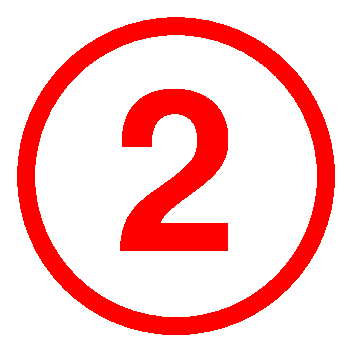
\includegraphics[scale=0.5,trim= 00 10 00 00]{../share/i/2.eps}
}

\newcommand{\TitlePicture}{%
\begin{center}%
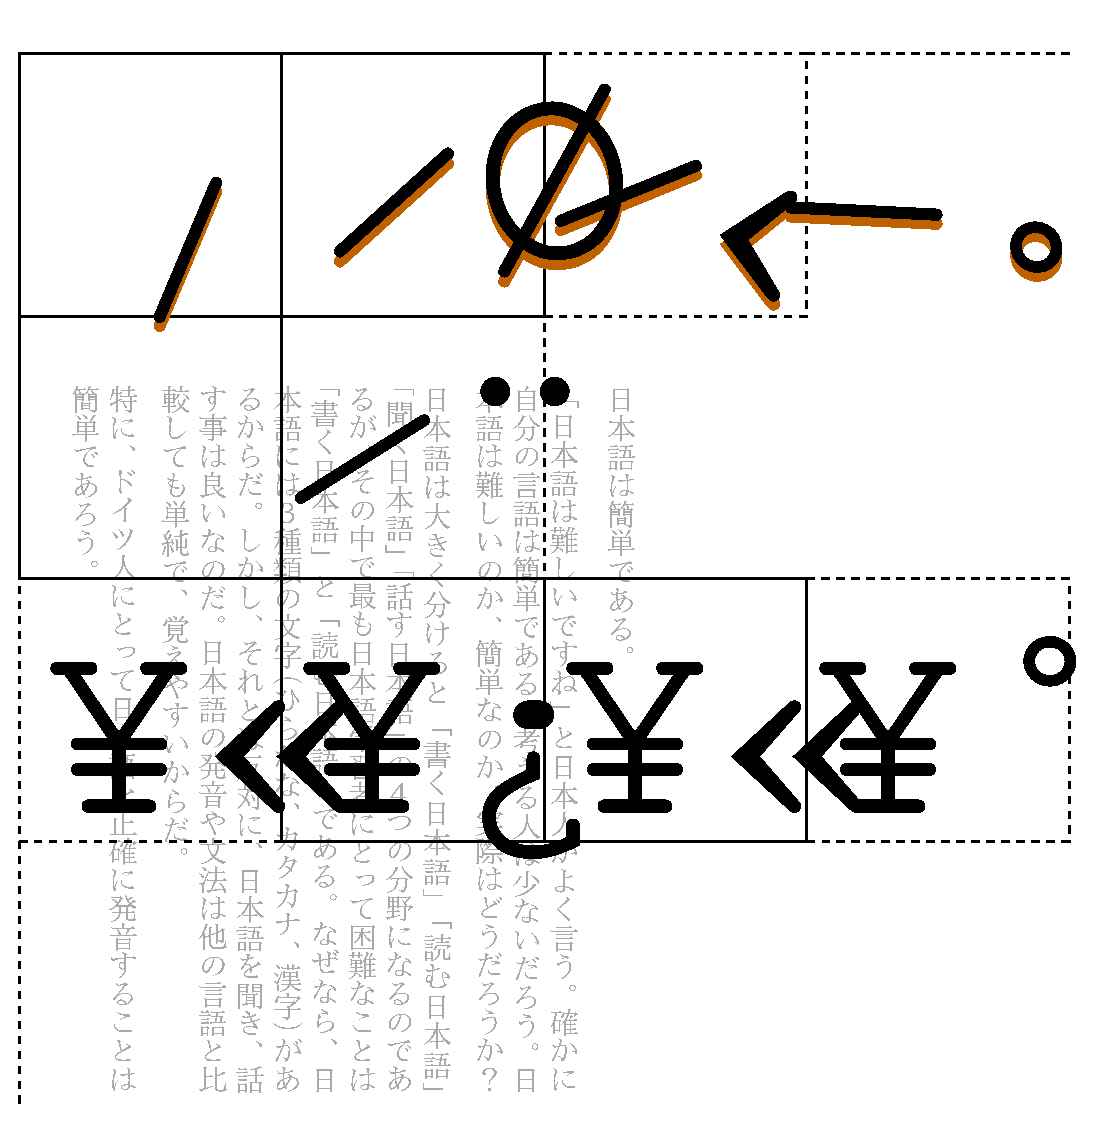
\includegraphics[scale=.5]{../share/i/kakikata-title-picture-600dpi.eps}%
\end{center}%
}%

\newcommand{\Kletter}[1]{%       l  b  r  t
\includegraphics[scale=0.95,trim=02 01 02 00]{../share/katakana/#1.pdf}
}

\newcommand{\KLETTER}[1]{%
\includegraphics[scale=2.0,trim= 00 05 00 00]{../share/katakana/#1.pdf}}

\newcommand{\Link}{ {
\includegraphics[scale=0.4,trim=00 00 01 00]{../share/i/link.pdf}} }


% PARAGRAPH COMMANDS
\newcommand{\Warn}[2]{
\begin{mdframed}[
linecolor=black!40,
outerlinewidth=1pt,
roundcorner=.5em,
innertopmargin=2ex,
innerbottommargin=.5\baselineskip,
innerrightmargin=1em,
innerleftmargin=1em,
backgroundcolor=blue!10,
%userdefinedwidth=1\textwidth,
shadow=true,
shadowsize=6,
shadowcolor=black!20,
frametitle={#1},
frametitlebackgroundcolor=red!40,
frametitlerulewidth=10pt
]

#2

\end{mdframed}
}
 % red   - additional dangerous info reg. lang
\newcommand{\Hint}[2]{
\bigskip
\relax
\begin{mdframed}[
linecolor=black!40,
outerlinewidth=1pt,
roundcorner=.5em,
innertopmargin=2ex,
innerbottommargin=.5\baselineskip,
innerrightmargin=1em,
innerleftmargin=1em,
backgroundcolor=blue!10,
%userdefinedwidth=1\textwidth,
shadow=true,
shadowsize=6,
shadowcolor=black!20,
frametitle={#1},
frametitlebackgroundcolor=blue!40,
frametitlerulewidth=10pt
]

#2

\end{mdframed}
}
 % blue  - additional important info reg. lang
% +---------------------------------------------------------------------------+
% | Info.tex                                                                  |
% |                                                                           |
% | Prints info box                                                           |
% |                                                                           |
% | Version: 0.1.1                                                            |
% |                                                                           |
% | Changes:                                                                  |
% |                                                                           |
% | 0.1.1 2020-07-23 Christian Kuelker <c@c8i.org>                            |
% |     - Add nobreak option as 3rd parameter (prevent page break)            |
% | 0.1.0 2014-08-24 Christian Kuelker <c@c8i.org>                            |
% |     - Initial release                                                     |
% |                                                                           |
% +---------------------------------------------------------------------------+


% needspace=6em:
%   https://tex.stackexchange.com/questions/201553/forbid-page-break-after-the-title-in-mdframed
%   https://kebo.pens.ac.id/CTAN/macros/latex/contrib/mdframed/mdframed-doc-en.pdf
\newcommand{\Info}[3]{
\bigskip
\relax
\begin{mdframed}[
linecolor=black!40,
outerlinewidth=1pt,
roundcorner=.5em,
innertopmargin=2ex,
innerbottommargin=.5\baselineskip,
innerrightmargin=1em,
innerleftmargin=1em,
backgroundcolor=blue!10,
%userdefinedwidth=1\textwidth,
shadow=true,
shadowsize=6,
shadowcolor=black!20,
needspace=12em,
frametitle={#1},
frametitlebackgroundcolor=green!40,
frametitlerulewidth=10pt,
nobreak=#3
]

#2

\end{mdframed}
}
 % green - additional important info
\newcommand{\Note}[2]{
\bigskip
\relax
\begin{mdframed}[
linecolor=black!40,
outerlinewidth=1pt,
roundcorner=.5em,
innertopmargin=2ex,
innerbottommargin=.5\baselineskip,
innerrightmargin=1em,
innerleftmargin=1em,
backgroundcolor=blue!10,
%userdefinedwidth=1\textwidth,
shadow=true,
shadowsize=6,
shadowcolor=black!20,
frametitle={#1},
frametitlebackgroundcolor=gray!40,
frametitlerulewidth=10pt
]

#2

\end{mdframed}
}
 % gray  - additional info
\newcommand{\Krow}[6]{
\begin{tabular}{|c|c|c|c|c|c|}\hline
\raisebox{.25\height}{
\includegraphics[scale=1.0,trim= 00 00 00 00]{../share/katakana/#1.pdf}
}
&\KLETTER{#2}&\KLETTER{#3}&\KLETTER{#4}&\KLETTER{#5}&\KLETTER{#6}\\\hline
\end{tabular}
}
 % 6 parameters
\newcommand{\Transcribe}[4]{
\begin{center}
\begin{tabular}{b{1cm}b{3cm}b{5cm}b{5cm}} 
#1 & #2 & #3 \rule[-10pt]{5cm}{.4pt} & #4 \\
\end{tabular}
\end{center}
}

\newenvironment{TranscribeEnv}{
\begin{minipage}{16cm}
\bigskip
\begin{center}
}{
\bigskip
\end{center}
\end{minipage}
}


\newcommand{\KatakanaSimpleTraining}[2]{

\bigskip

Please transcribe the following words from \textbf{#1}:

\fbox{
\begin{TranscribeEnv}
#2
\end{TranscribeEnv}
}
}

%CharacterExplanation{soexplanation}{TEXT}

\newcommand{\CharacterExplanation}[2]{

\bigskip

\begin{tabular}{cc}
\raisebox{-.5\height}{\KLETTER{#1}} &
\begin{minipage}{13cm}
#2
\end{minipage}\\
\end{tabular}

\bigskip

}


% PAGE COMMANDS
\newcommand{\KatakanaTraining}[1]{%

\bigskip Draw slowly, precise and try to make it beautiful. One line per day.

\begin{tabular}{|c|c|c|c|c|c|}\hline
\KLETTER{#1s}&\KLETTER{#1}&\KLETTER{#1g}&\KLETTER{ar}&\KLETTER{s}\\\hline
\KLETTER{s}&\KLETTER{s}&\KLETTER{s}&\KLETTER{s}&\KLETTER{s}\\\hline
\KLETTER{s}&\KLETTER{s}&\KLETTER{s}&\KLETTER{s}&\KLETTER{s}\\\hline
\end{tabular}

\bigskip Slowly from top to bottom. Precise and take care about the stroke
order. One column per hour, maximum four columns per day.

\begin{tabular}{|c|c|c|c|c|c|c|c|c|c|c|c|}\hline
\Kletter{s}&\Kletter{s}&\Kletter{s}&\Kletter{s}&\Kletter{s}&
\Kletter{s}&\Kletter{s}&\Kletter{s}&\Kletter{s}&\Kletter{#1}\\\hline
&&&&&&&&&\Kletter{#1g}\\\hline
&&&&&&&&&\Kletter{ad}\\\hline
&&&&&&&&&\Kletter{s}\\\hline
&&&&&&&&&\Kletter{s}\\\hline
\end{tabular}
\newpage

Write faster from left to right. If one character is wrong continue with slower
speed.

\begin{tabular}{|c|c|c|c|c|c|c|c|c|c|c|c|}\hline
\Kletter{#1s}&\Kletter{#1}&\Kletter{#1g}&\Kletter{ar}&\Kletter{s}&
\Kletter{s}&\Kletter{s}&\Kletter{s}&\Kletter{s}&\Kletter{s}\\\hline
&&&&&&&&&\Kletter{s}\\\hline
&&&&&&&&&\Kletter{s}\\\hline
&&&&&&&&&\Kletter{s}\\\hline
&&&&&&&&&\Kletter{s}\\\hline
&&&&&&&&&\Kletter{s}\\\hline
\end{tabular}

\bigskip Repeat the training after a week in medium pace.

\begin{tabular}{|c|c|c|c|c|c|c|c|c|c|c|c|}\hline
\Kletter{s}&\Kletter{s}&\Kletter{s}&\Kletter{s}&\Kletter{s}&
\Kletter{s}&\Kletter{s}&\Kletter{s}&\Kletter{s}&\Kletter{#1}\\\hline
&&&&&&&&&\Kletter{#1g}\\\hline
&&&&&&&&&\Kletter{ad}\\\hline
&&&&&&&&&\Kletter{s}\\\hline
&&&&&&&&&\Kletter{s}\\\hline
&&&&&&&&&\Kletter{s}\\\hline
&&&&&&&&&\Kletter{s}\\\hline
\end{tabular}
\newpage
}

\newcommand{\KatakanaHeader}[2]{%
\begin{tabular}{clr}
\raisebox{-.5\height}{\includegraphics[scale=1.0,trim= 00 00 00 00]{../share/katakana/#1t.pdf}} &
\begin{minipage}{12.5cm}
#2
\end{minipage}&
\raisebox{-.4\height}{\includegraphics[scale=2.0,trim= 00 05 00 00]{../share/katakana/#1s.pdf}} 
\\
\end{tabular}
}


% TITLE
% ===========================================================================
% TITLE
% ===========================================================================
\author{\AuthorName}
\title{ \NumberTwo\\
    The Japanese Script \\ \texttt{日本語の書き方}\\
    \bigskip \large Katakana \\ \texttt{片仮名}
}
\date{ \TitlePicture \footnotesize \jdate, v-\jversion }
\dedication{to Francesco Belletti}
\uppertitleback{ \footnotesize

Copyright \copyright~ 2000, 2001, 2002, 2003, 2004, 2005, 2006, 2013, 2014 by
\href{mailto:christian.kuelker@cipworx.org}{Christian K\"ulker}.

\medskip

See the web page 
\href{http://christian.kuelker.info/nihongo/}{http://christian.kuelker.info/nihongo/}

%” ”
%"

Permission is granted to copy, distribute and/or modify this document under the
terms of the GNU Free Documentation License (GNU-FDL), version 1.2 or any later
version published by the Free Software Foundation; with no invariant sections
except the following invariant back-cover text (see framed box below:
\textit{Back-Cover Text}).

A copy of the license is included in the section entitled ”GNU Free
Documentation License”. 

\normalsize
}
\lowertitleback{     \begin{center}
        \textbf{Back-Cover Text:}
        \begin{tabular}{|l|}\hline
            \begin{minipage}{140mm}\medskip

                The original version of this book was written by
                \textbf{Christian Külker} and is copyrighted 2000-2006,
                2013-2014 under the GNU-FDL version 1.2 or any later version
                published by the Free Software Foundation with only this
                section as invariant section. \medskip

                The version v0.1 - v0.8 of this book \textbf{日本語を書こう!}
                (German: \textit{Lasst uns Japanisch schreiben!}) was developed
                as reference and training book for the language course at the
                VHS Halle (Ravensberg) in Germany starting year 2000. It was
                published 2003, 2004 and 2006 under the GNU FDL.\medskip

                In 2014 (v0.9) the part of Katakana was made a book on its own.
                The title was changed to \textbf{日本語の書き方:片仮名}
                (English: \textit{The Japanese Script - Katakana}) and adopted
                to a self study approach.\medskip

                In 2020 (v1.0) the source code was changed to compile under
                Debian 10 Buster. Some fonts have been changed in the
                appendix.

                \medskip

                Original PDF:
                \href{https://github.com/ckuelker/nihongo/tree/master/pub/}{https://github.com/ckuelker/nihongo/tree/master/pub}

                Source Code:
                \href{https://github.com/ckuelker/nihongo/}{https://github.com/ckuelker/nihongo}

                Web site:
                \href{https://christian.kuelker.info/nihongo/}{https://christian.kuelker.info/nihongo}


                \flushright  Christian Külker, Bielefeld, \jdate, \texttt{v-\jversion}

                \medskip

            \end{minipage}\\ \hline
        \end{tabular}
    \end{center}
    \bigskip

%    \texttt{v1.0}: Appendix fonts changed.

%    \texttt{v0.9}: Initial version as Katakana only book.

%    In case you have the original book, please write to
%    \href{mailto:christian.kuelker@cipworx.org}{christian.kuelker@cipworx.org}
%    for hints, suggestions, thanks, complains.

}


% ===========================================================================
% DOCUMENT
% ===========================================================================
\begin{document}
\pagestyle{plain}
\frontmatter
\maketitle

% CONTENTS
\tableofcontents
\pagestyle{fancy}

\mainmatter

% ===========================================================================
\chapter{片仮名 - Katakana}

\Warn{Warning!}{This work is a \textbf{draft}. It is not complete and contains
errors. Please report.}

\bigskip

The second Japanese Kana script, \hyperref[sec:Syllable]{syllable}, better
\hyperref[sec:Mora]{morae} based writing system is called Katakana and written
in Japanese as {片仮名} {【かたかな】} but sometimes also as {カタカナ}.  It
consists of a littel less the 50 letters, as it is usual for morae baseed
systems and it derived from Chinese characters, called Kanji
{漢字} {【かんじ】} in Japanese. Together they form a complete phonetic
script. 

Even though Katakana can be used by its own to express the complete content of
the Japanese language it is almost never used as such.This is due to the fact
that the other two scripts Hiragana and Kanji exists and that there was
traditionally no space character to separate words. So a Katakana sentence with
Katakana only and no spaces is hardly understandable due to many homophones.
But even if there are spaced it is difficult. Therefore the letter type
boundaries of Kanji, Hirangana and Katakana are the most significant indicator
for word boundaries. 

In the Japanese written language Katakana has a destricnt role. It serves for:

\begin{tabular}{rl}
1.& writing words of foreign origin\\
2.& words that need to be emphasized\\
3.& botanic names\\
4.& faunic names\\
5.& partly onomatopoeias in Manga\\	
\end{tabular}

\section{Pronunciation and Intonation}

The pronunciation of Katakana is the same as for Hiragana. Therefore every
syllable, more precise every mora corresponds to a Katakana character and is
constructed as 'consonant' + 'vowel' with the exception of |n|. This system of
letter for each mora makes pronunciation absolutely clear with no
ambiguities. However the simplicity of Katakana does not mean that
pronunciation in Japanese is simple for English speakers as it is for Germans. 
The rigid structure of the fixed mora sound in Japanese creates the challenge 
of learning the proper intonation and duration of Japanese pronunciation. 

Almost each Japanese word can be chunked into morae of high and low pitch witch
is a crucial aspect of the spoken language. Compared to Chinese, Japanese
luckily have only two pitched: hi and low. Sometimes this difference can be
even important for the lexic. Homophones can have for example a difference in
pitch which make them distinguishable.  The intonation of high and low pitches
is a crucial aspect of the spoken language. One of the biggest problems for
obtaining a natural sounding pronunciation is the incorrect intonation. Many
European or American learners speak without paying attention to the correct
pitch. That makes the speech sound non-natural for Japanese. In some language
course try to let the learner memorize the natural pitch of a word or even
teach rules for memorization. While there is clearly a possibility for
linguistic rules, they are hard to remember and master. Also because they can
remember the rules it is still possible to learn the correct intonation by
resorting to language learning techniques used by infants or small children:
mimicking native Japanese speakers. Therefore it is highly adviced to expose
oneself to as many Japanese spoken language as possible and to mimic it. Radio,
podcasts, drama and television to name a few. However, it is not adviced to
listen too much artificial sources like anime or commercials.  

\begin{tabular}{rl}
-&every (yes \textbf{every}) mora is pronounced with the same length\\
-&there is no short and long mora or letters\\
-&every mora has a pich: high or low\\
-&every pitch matters\\
-&the pitch can change with its context\\
-&the pitch can change with a dialect - however well defined in standard Japanese\\
\end{tabular}

\section{Writing Katakana}

Writing Katakana is not much different as writing Hiragana. Katakana is written
mostly from left to right and up to down. In some texts from up to up to down
and right to left. 

\bigskip

\begin{tabular}{p{4cm}p{4cm}p{4cm}m{4cm}}
horizontally&
\fbox{
\begin{minipage}{3.2cm}
コノテクトハゼンブデカタカナデカカレタモノデアル。カタカナダケデカクト、カナリヨミニクイテクトトナリマス。
\end{minipage}
}
& vertically &
%\setCJKfamilyfont{cjk-vert}[Script=CJK,RawFeature=vertical]{Kozuka Gothic Pro M}
\setCJKfamilyfont{cjk-vert}[Script=CJK,RawFeature=vertical]{IPAPGothic}
\raisebox{-.5\height}{
\fbox{
\rotatebox{-90}{
\begin{minipage}{3.2cm} \CJKfamily{cjk-vert}
コノテクトハゼンブデカタカナデカカレタモノデアル。
カタカナダケデカクト、カナリヨミニクイテクトトナリマス。
\end{minipage}
}
}
}
\\
\end{tabular}
\bigskip

Even if it possible to change the orientation the letter as such is \textbf{not} rotated.

% ===========================================================================
\chapter{片仮名練習 - Katakana Training}

todo
\newpage

%----------------------------------------------------------------------------
\section{Katakana /a/ Row -  片仮名ア行}\label{sec:KatakanaARow}

\Krow{arow}{a}{i}{u}{e}{o}

\label{letter:a}\KLETTER{a} The 片仮名 {「ア」} derives from the
\hyperref[sec:PhoneticCharacter]{Phonetic Caracters}
(\hyperref[sec:Radical]{radical}).  A smaller version {「ァ」} is used in
combinations with other letters as {「ファ」} and is pronounced as /fa/ in
\hyperref[sec:Hepburn]{Hepburn} transcription.

\label{letter:u}\KLETTER{i} The 片仮名 {「イ」} derives from the
\hyperref[sec:PhoneticCharacter]{Phonetic Caracters} {「伊」} left element
(\hyperref[sec:Radical]{radical}).  A smaller version {「ィ」} is used in
combinations with other letters and represents a
\hyperref[sec:Diphthong]{diphthong}. 

\label{letter:u}\KLETTER{u} The 片仮名 {「ウ」} derives from the
\hyperref[sec:PhoneticCharacter]{Phonetic Caracter} {「宇」}. A smaller version
{「ゥ」} is used in combinations with other letters and represents a
\hyperref[sec:Diphthong]{diphthong} and is written as "w". Even though the
combination {「トゥ」} /tu/ exist, it is relatively new and many words do not
use it. In this cases {「ツ 」} /tsu/ is used. {「ウ」} can take
\hyperref[sec:Dakuten]{Dakuten} to form {「ヴ」} /vu/, which is relatively new
and can replace {「ブ」} /bu/. 

\Note{Note}{%

Be aware that the characters \hyperref[letter:fu]{「フ」},
\hyperref[letter:wa]{「ワ」}  and \hyperref[letter:u]{「ウ」} look very
similar.  Make sure that you spend extra training on distinguish them. 

}%


\newpage 

\label{letter:e}\KLETTER{e} The 片仮名 {「エ」} derives from the
\hyperref[sec:PhoneticCharacter]{Phonetic Caracters} {「江」} right element
(\hyperref[sec:Radical]{radical}). A smaller version {「ェ」} is used in
combinations with other letters and express \hyperref[sec:Mora]{morae} of
foreign origin. For example {「ヴェ」} as pronounced /ve/.

\label{letter:o}\KLETTER{o} The 片仮名 {「オ」} derives from the
\hyperref[sec:PhoneticCharacter]{Phonetic Caracter} {「於」}. A smaller version
{「ォ」} is used in combinations with other letters and express
\hyperref[sec:Mora]{morae} of foreign origin. For example {「フォ 」} as
pronounced /fe/.

\newpage

% ---------------------------------------------------------------------------
\subsection{/a/ - 「ア」} \label{sec:KatakanaA}

\KatakanaHeader{a}{ The Katakana {「ア」} is written with two strokes. The
first stroke starts horizontal. The second stroke is a curve with can be
attached to the first stroke in hand writing, but not at the horizontal part -
at the end of the first line.} \KatakanaTraining{a}

% ---------------------------------------------------------------------------
\subsection{/i/ - 「イ」} \label{sec:KatakanaI}

\KatakanaHeader{i}{ The Katakana {「イ」} is written with one stroke. The first
stroke is a curve from upper right to lower left. The second stroke is a
vertical line attached to the first at the top.} \KatakanaTraining{i}

% ---------------------------------------------------------------------------
\subsection{/u/ - 「ウ」} \label{sec:KatakanaU}

\KatakanaHeader{u}{The Katakana {「ウ」} is written with three strokes. The
first stroke a small vertical line. The second a small vertical line again and
the third line a horizontal line connection the two others.}
\KatakanaTraining{u}

% ---------------------------------------------------------------------------
\subsection{/e/ - 「エ」} \label{sec:KatakanaE}

\KatakanaHeader{e}{The Katakana {「エ」} is written with three strokes. It is
very geometrically consisting only out of horizontal and vertical lines
connected together.} \KatakanaTraining{e}

% ---------------------------------------------------------------------------
\subsection{/o/ - 「オ」} \label{sec:KatakanaO}

\KatakanaHeader{o}{The Katakana {「オ」} is written with three strokes. The
first line is horizontal and together with the second stroke it constructs a
perfect crossing. The third stroke beginning lies at the center of the
crossing.} \KatakanaTraining{o}

% ---------------------------------------------------------------------------
\section{/a/ Row Training - 片仮名ア行練習}
\Padding
\begin{longtable}[c]{p{2cm}p{2cm}p{3cm}p{6cm}p{2cm}}
\textit{Katakana}&\textit{Rōmaji}&\textit{Original}&\textit{Remark}&Origin\\\hline
ウエア&wuea&ware&          &English\\
エア  &ea  &air &          &English\\
エイ  &ei  &A   &the letter&English\\
\end{longtable}

\KatakanaSimpleTraining{Katakana to Romaji}{
\Transcribe{1.}{ウエア}{}{wear, ware}
\Transcribe{2.}{エア}{}{air}
\Transcribe{3.}{エイ}{}{A (the letter)}
\Transcribe{4.}{アイ}{}{I (the letter)}
\Transcribe{5.}{オウ}{}{O (the letter)}
%\Transcribe{6.}{イア}{}{ear}
}

\KatakanaSimpleTraining{Romaji to Katakana}{
\Transcribe{1.}{ea}{}{air}
\Transcribe{2.}{ai}{}{I (the letter)}
\Transcribe{3.}{ou}{}{O (the letter)}
\Transcribe{4.}{ei}{}{A (the letter)}
\Transcribe{5.}{uea}{}{wear, ware}
%\Transcribe{6.}{ia}{}{ear}
}

\newpage
\Padding
\begin{longtable}[c]{p{2cm}p{2cm}p{3cm}p{6cm}p{2cm}}
\textit{Katakana}&\textit{Rōmaji}&\textit{Original}&\textit{Remark}&Origin\\\hline
アイ  &ai  &I   &the letter&English\\
オウ  &ou  &O   &the letter&English\\
イア  &ia  &ear &          &English\\
\end{longtable}

\KatakanaSimpleTraining{English to Romaji}{
\Transcribe{1.}{ear}{}{}
\Transcribe{2.}{I (the letter)}{}{}
\Transcribe{3.}{air}{}{}
\Transcribe{4.}{O (the letter)}{}{}
\Transcribe{5.}{wear, ware}{}{}
%\Transcribe{6.}{A (the letter)}{}{}
}

\KatakanaSimpleTraining{English to Katakana}{
\Transcribe{1.}{I (the letter)}{}{}
\Transcribe{2.}{O (the letter)}{}{}
\Transcribe{3.}{air}{}{}
\Transcribe{4.}{ear}{}{}
\Transcribe{5.}{wear, ware}{}{}
%\Transcribe{6.}{A (the letter)}{}{}
}
\newpage
   % OK
% ---------------------------------------------------------------------------
\section{Katakana /ka/ Row}\jsec{片仮名 カ行}\label{sec:KatakanaKaRow}

\Krow{karow}{ka}{ki}{ku}{ke}{ko}

\label{letter:ka}\KLETTER{ka} The  片仮名 {「カ」} is pronounced  /ka/ and  derives from the
\hyperref[sec:PhoneticCharacter]{Phonetic Character}s {「加」} left
\hyperref[sec:Radical]{radical}.  A \hyperref[sec:Dakuten]{濁点} version exists
and pronounced as /ga/.

%\hyperref[sec:Handakuten]{半濁点} does not exist in daily Japanese.  
% {「一ヵ所」} {【いちかしょ】} (one place)
% {「一ヶ所」} {【いちかしょ】} (one place).
% 十ヵ条(十ヶ条)


\Note{Note}{A smaller version {「ヵ」} is rare but used in combinations with
number particles.  For example in {「一ヵ月」} {【いっかげつ】} (one month) and
others.  This cases can also be written {「一ヶ月」} {【いっかげつ】} (one
month). Please see also \nameref{sec:KatakanaKe}. \Link
\href{https://ja.wikipedia.org/wiki/\%E3\%83\%B5}{ヵ} }

\label{letter:ki}\KLETTER{ki} The 片仮名 {「キ」} derives from the
\hyperref[sec:PhoneticCharacter]{Phonetic Character}s middle part of either {「機」} or
{「幾」}.  It is pronounced as /ki/.  A \hyperref[sec:Dakuten]{濁点} version
exists and pronounced as /gi/.


\label{letter:ku}\KLETTER{ku} The 片仮名 {「ク」} derives from the
\hyperref[sec:PhoneticCharacter]{Phonetic Character}s left upper part of {「久」}.  It
is pronounced as /ku/.  A \hyperref[sec:Dakuten]{濁点} version exists and
pronounced as /gu/.  A smaller version exists, but is used for the Ainu
Language.



\label{letter:ke}\KLETTER{ke} The 片仮名 {「ケ」} derives from the
\hyperref[sec:PhoneticCharacter]{Phonetic Character}s upper and left part of {「介」}.
It is pronounced as /ke/.  A \hyperref[sec:Dakuten]{濁点} version exists and
pronounced as /ge/.  The smaller version {「ヶ」} is explained in the following
note.

\newpage

\Note{Note}{ A smaller version {「ヶ」} is rare but used in combinations with
number particles.  For example in {「一ヶ月」} {【いっかげつ】} (one month) and
others.  This cases can also be written {「一ヵ月」} {【いっかげつ】} (one
month). There are cases where only {「ヶ」} can be written {七ヶ宿}
{【シチカシュク】} (Place at the south west border of the prefecture Miyagi).
In other rare cases this character can be pronounced different {「関ヶ原」}
{【せきがはら】} (Place at the south border of the Gifu prefecture, known by
the battle at 1600.). Please see also \nameref{sec:KatakanaKa}. \Link
\href{https://ja.wikipedia.org/wiki/\%E3\%83\%B5}{ヵ} }

\label{letter:ko}\KLETTER{ko} The 片仮名 {「コ」} derives from the
\hyperref[sec:PhoneticCharacter]{Phonetic Character}s upper part of {「己」}.  It is
pronounced as /ko/.  A \hyperref[sec:Dakuten]{濁点} version exists and
pronounced as /go/.



\newpage

% ---------------------------------------------------------------------------
\subsection{/ka/}\jsubsec{「カ」} \label{sec:KatakanaKa}

\KatakanaHeader{ka}{ /ka/ is written with 2 strokes. Basically the same way as
the Hiragana {「か」} it looks like a squarish version, but without the last
stroke. The hook at the second stroke is less significant or important.  }
\KatakanaTraining{ka}

% ---------------------------------------------------------------------------
\subsection{/ki/}\jsubsec{「キ」} \label{sec:KatakanaKi}

\KatakanaHeader{ki}{ The shape alignment of the 「キ」character is not straight
towards its environment. However the junctions are more or less 90 degrees.  }
\KatakanaTraining{ki}

% ---------------------------------------------------------------------------
\subsection{/ku/}\jsubsec{「ク」} \label{sec:KatakanaKu}
% ---------------------------------------------------------------------------

\KatakanaHeader{ku}{ The first stroke is similar the stroke of {「ケ 」} is a
curve. While the second stroke start aligned and straight. }
\KatakanaTraining{ku}

% ---------------------------------------------------------------------------
\subsection{/ke/}\jsubsec{「ケ」} \label{sec:KatakanaKe}

\KatakanaHeader{ke}{ The {「ケ 」} is written with 3 strokes and the first
stroke is similar to the {「ク」}. The second stroke is aligned and straight.
While the last stroke is a curve.  } \KatakanaTraining{ke}

% ---------------------------------------------------------------------------
\subsection{/ko/}\jsubsec{「コ」} \label{sec:KatakanaKo}

\KatakanaHeader{ko}{ This character is almost a geometric figure composed out
of two strokes. However unless in European languages this are only 2 strokes
and not 3. The first stroke is the longest one and done similar with all
{漢字}. } \KatakanaTraining{ko}

% ---------------------------------------------------------------------------
\subsection{/ka/ Row Training}\jsubsec{片仮名カ行練習}

\Padding
\begin{longtable}[c]{p{2cm}p{1.5cm}p{1.5cm}p{3cm}p{7cm}}
\textit{Katakana}&\textit{Rōmaji}&\textit{Original}&\textit{Remark}&Origin\\\hline
カキ  &kaki &kaki &柿 persimon&Japanese\\
ケア  &kea  &care &          &English\\
ケイ  &kei  &K    &the letter&English\\
\end{longtable}

\KatakanaSimpleTraining{Katakana to Rōmaji}{
\Transcribe{1.}{カキ}{}{persimmon}
\Transcribe{2.}{ココア}{}{cocoa}
\Transcribe{3.}{ケア}{}{care}
\Transcribe{4.}{コア}{}{core}
\Transcribe{5.}{ケーキ}{}{cake}
%\Transcribe{6.}{ケイ}{}{K (the letter)}
}

\KatakanaSimpleTraining{Rōmaji to Katakana}{
\Transcribe{1.}{kokoa}{}{cocoa}
\Transcribe{2.}{k$\overline{\mbox{e}}$ki}{}{cake}
\Transcribe{3.}{kea}{}{care}
\Transcribe{4.}{koa}{}{core}
\Transcribe{5.}{kaki}{}{persimmon}
%\Transcribe{6.}{kei}{}{K (the letter)}
}

\newpage

\Padding
%\begin{longtable}[c]{p{2cm}p{2cm}p{3cm}p{6cm}p{2cm}}
\begin{longtable}[c]{p{2cm}p{2.0cm}p{3.5cm}p{4cm}p{2.5cm}}
\textit{Katakana}&\textit{Rōmaji}&\textit{Original}&\textit{Remark}&Origin\\\hline
コア  &koa  &core &          &English\\
ココア&kokoa&cocoa& hot chocolate &English, from metathesis of Spanish cacao, from Nahuatl cacahuatl\\
ケーキ&kēki &cake &          &English\\
\end{longtable}


\KatakanaSimpleTraining{English to Rōmaji}{
\Transcribe{1.}{persimon}{}{}
\Transcribe{2.}{cocoa}{}{}
\Transcribe{3.}{care}{}{}
\Transcribe{4.}{core}{}{}
\Transcribe{5.}{K (the letter)}{}{}
%\Transcribe{6.}{cake}{}{}
}

\KatakanaSimpleTraining{English to Katakana}{
\Transcribe{1.}{cocoa}{}{}
\Transcribe{2.}{cake}{}{}
\Transcribe{3.}{care}{}{}
\Transcribe{4.}{persimon}{}{}
\Transcribe{5.}{K (the letter)}{}{}
%\Transcribe{6.}{core}{}{}
}

\newpage
  % OK
%----------------------------------------------------------------------------
\section{Katakana /sa/ Row}\jsec{片仮名サ行}\label{sec:KatakanaSaRow}

\Krow{sarow}{sa}{shi}{su}{se}{so}

\label{letter:sa}\KLETTER{sa} The  片仮名 {「サ」} is pronounced  /sa/ and
derives from the \hyperref[sec:PhoneticCharacter]{Phonetic Character}s {「散」}
upper left corner \hyperref[sec:Radical]{radical}.  A
\hyperref[sec:Dakuten]{濁点} version exists and pronounced as /za/.

\label{letter:shi}\KLETTER{shi} The 片仮名 {「シ」} derives from the
\hyperref[sec:PhoneticCharacter]{Phonetic Character}  {「之 」}.  It is
pronounced as /shi/.  A \hyperref[sec:Dakuten]{濁点} version exists and
pronounced as /ji/.

\Note{Note}{Please see section \nameref{subsec:ShiTsuAmbiguity} for the
explanation how to write and distinguish /shi/ and /tsu/.  }

\label{letter:su}\KLETTER{su} The 片仮名 {「ス」} derives from the
\hyperref[sec:PhoneticCharacter]{Phonetic Character}s right lower part of
{「須」}.  It is pronounced as /su/.  A \hyperref[sec:Dakuten]{濁点} version
exists and pronounced as /zu/.

\label{letter:se}\KLETTER{se} The 片仮名 {「セ」} derives from the
\hyperref[sec:PhoneticCharacter]{Phonetic Character}s middle left part of
{「世」}.  It is pronounced as /se/.  A \hyperref[sec:Dakuten]{濁点} version
exists and pronounced as /ze/.

\newpage

\label{letter:so}\KLETTER{so} The 片仮名 {「ソ」} derives from the
\hyperref[sec:PhoneticCharacter]{Phonetic Character}s upper right part of
{「曽」}.  It is pronounced as /so/.  A \hyperref[sec:Dakuten]{濁点} version
exists and pronounced as /zo/.

% SoRiNAmbiguity
\subsection{|so|, |ri| and |n| Ambiguity} \label{subsec:SoRiNAmbiguity}

The Katakana characters {「ソ」}, {「リ」} and {「ン」} can be difficult to
distinguish. All three are made out of only 2 strokes. And especially |so| and
|n| can be hard to tell. In a sentence of course the context can help a lot.
But what are the rules for this characters to write properly and distinguish?

\bigskip

\begin{center}
\begin{tabular}{|c|c|c|}\hline
\KLETTER{so}&\KLETTER{n}&\KLETTER{ri}\\\hline
\end{tabular}
\end{center}

\CharacterExplanation{soexplanation}{ To write the letter |so| it is important
to align both lines \textbf{horizontally} (red line) and to \textbf{non-align}
the ends (blue line) vertically. In this way it is possible to distinguish |so|
from |n|, but not from |ri|. To also distinguish it from |ri| you have to write
the first stroke not horizontally nor vertically (green line).  }

\CharacterExplanation{nexplanation}{ To write the letter |n| it is important to
a align both lines \textbf{vertically} (red line) and to \textbf{non-align} the
ends (blue line). In this way it is possible to distinguish |n| from |so|. If
both lines are aligned there should not be a problem to distinguish it from
|ri|. Usually the angle of the green line is different, but only a small
indicator. }

\CharacterExplanation{riexplanation}{ To write the letter |ri| it is important
to \textbf{align} both of the line beginnings \textbf{horizontally} (red line)
and to make sure that both lines are \textbf{parallel} (green lines). There
should be \textbf{no alignment} on the left side (blue line)
\textbf{vertically}. The difference between |so| and |ri| is that |ri| need to
start with two \textbf{parallel} lines wile |so| should not. Please compare the
left green line for an explanation.  }



\newpage
% ---------------------------------------------------------------------------
\subsection{/sa/}\jsubsec{「サ」}\label{sec:KatakanaSa}

\KatakanaHeader{sa}{ Katakana {「サ」} is written with three strokes. All
crossings of strokes are in a 90 degree angle.  The starts of all strokes are
aligned eitehr horizontally or vertically. The last stroke has a curve.}
\KatakanaTraining{sa}

% ---------------------------------------------------------------------------
\subsection{/shi/}\jsubsec{「シ」}\label{sec:KatakanaShi}

\KatakanaHeader{shi}{ The Katakana {「シ」} is written with three strokes. All
three strokes are aligned vertically in the beginning. Please see section
\nameref{subsec:ShiTsuAmbiguity}.} \KatakanaTraining{shi}

% ---------------------------------------------------------------------------
\subsection{/su/}\jsubsec{「ス」}\label{sec:KatakanaSu}

\KatakanaHeader{su}{The Katakana {「ス」} is written with two strokes. The
first stroke startes horizontally aligned. The second stroke touches the first
stroke at the beginning.} \KatakanaTraining{su}

% ---------------------------------------------------------------------------
\subsection{/se/}\jsubsec{「セ」}\label{sec:KatakanaSe}

\KatakanaHeader{se}{ The Katakana {「セ」} is written with two strokes. The
crossing has \textbf{no} 90 degree angle. The curve of the second stroke as
almost a 90 deegre angle. } \KatakanaTraining{se}

% ---------------------------------------------------------------------------
\subsection{/so/}\jsubsec{「ソ」}\label{sec:KatakanaSo}

\KatakanaHeader{so}{ The Katakana {「ソ」} is written with two strokes. The
first stroke is not aligned verticall but it is aligned horizontally withe the
second stroke. Please see section \nameref{subsec:SoRiNAmbiguity}.}
\KatakanaTraining{so}

% ---------------------------------------------------------------------------
\subsection{/sa/ Row Training}\jsubsec{片仮名サ行練習}\label{sec:SaRowTraining}
% 3 78 エキス
%3 357 スカイ
%3 360 スキー
%3 3 アイス
%3 111 ガーゼ
%3 146 イエス
\Padding
\begin{longtable}[c]{p{2cm}p{2cm}p{3cm}p{6cm}p{2cm}}
\textit{Katakana}&\textit{Rōmaji}&\textit{Original}&\textit{Remark}&\textit{Origin}\\\hline
エキス&ekisu&ex(tract)&extract&Dutch\\
スカイ&sukai&sky&&English\\
スキー&sukī&ski&noun for skiing&English\\
\end{longtable}
\KanaSimpleTraining{Katakana to Rōmaji}{
\Transcribe{1.}{エキス}{}{extract}      % ekisu
\Transcribe{2.}{スカイ}{}{sky}          % sukai
\Transcribe{3.}{スキー}{}{ski}          % sukī
\Transcribe{4.}{アイス}{}{ice}          % aisu
\Transcribe{5.}{ガーゼ}{}{gauze}        % gāze
%\Transcribe{6.}{イエス}{}{Jesus}        % iesu
}

\KanaSimpleTraining{Rōmaji to Katakana}{
\Transcribe{1.}{sukai}{}{sky}         % sukai
\Transcribe{2.}{ekisu}{}{extract}     % ekisu
\Transcribe{3.}{aisu}{}{ice}          % aisu
\Transcribe{4.}{suki}{}{ski}          % sukī
\Transcribe{5.}{iesu}{}{Jesus}        % iesu
%\Transcribe{6.}{gāze}{}{gauze}        % gāze
}

\newpage

\Padding
\begin{longtable}[c]{p{2cm}p{2cm}p{3cm}p{6cm}p{2cm}}
\textit{Katakana}&\textit{Rōmaji}&\textit{Original}&\textit{Remark}&Origin\\\hline
アイス&aisu&ice&water ice, ice cream&English\\
ガーゼ&gāze&Gaze&gauze&German\\
イエス&iesu&Jesus&Jesus&Portuguese\\
\end{longtable}
\KanaSimpleTraining{English to Rōmaji}{
\Transcribe{1.}{extract}{}{}       % ekisu
\Transcribe{2.}{sky}{}{}           % sukai
\Transcribe{3.}{Jesus}{}{}         % iesu
\Transcribe{4.}{gauze}{}{}         % gāze
\Transcribe{5.}{ice}{}{}           % aisu
%\Transcribe{6.}{ski}{}{}           % sukī
}

\KanaSimpleTraining{English to Katakana}{
\Transcribe{1.}{sky}{}{}           % sukai
\Transcribe{2.}{gauze}{}{}         % gāze
\Transcribe{3.}{ice}{}{}           % aisu
\Transcribe{4.}{Jesus}{}{}         % iesu
\Transcribe{5.}{extract}{}{}       % ekisu
%\Transcribe{6.}{ski}{}{}           % sukī
}

\newpage
  % OK
% ---------------------------------------------------------------------------
\section{Katakana /ta/ Row}\jsec{片仮名タ行}\label{sec:KatakanaTaRow}

\Krow{tarow}{ta}{chi}{tsu}{te}{to}

\label{letter:ta}\KLETTER{ta} The  片仮名 {「タ」} is pronounced  /ta/ and
derives from the \hyperref[sec:PhoneticCharacter]{Phonetic Character}s {「多 」}
upper or lover \hyperref[sec:Radical]{radical}.  A \hyperref[sec:Dakuten]{濁点}
version exists and pronounced as /da/.

\label{letter:chi}\KLETTER{chi} The 片仮名 {「チ」} derives from the
\hyperref[sec:PhoneticCharacter]{Phonetic Character}  {「千」}.  It is
pronounced as /chi/.  A \hyperref[sec:Dakuten]{濁点} version exists and
pronounced as /ji/.

\label{letter:tsu}\KLETTER{tsu} The 片仮名 {「ツ」} derives from the
\hyperref[sec:PhoneticCharacter]{Phonetic Character}s {「州」} or {「川」} .  It
is pronounced as /tsu/.  A \hyperref[sec:Dakuten]{濁点} version exists and
pronounced as /zu/. 

\label{letter:te}\KLETTER{te} The 片仮名 {「テ」} derives from the
\hyperref[sec:PhoneticCharacter]{Phonetic Character}s lower left part of {「天
」}.  It is pronounced as /te/.  A \hyperref[sec:Dakuten]{濁点} version exists
and pronounced as /de/.  

\newpage

\label{letter:to}\KLETTER{to} The 片仮名 {「ト」} derives from the
\hyperref[sec:PhoneticCharacter]{Phonetic Character}s right part of {「止」}.
It is pronounced as /to/.  A \hyperref[sec:Dakuten]{濁点} version exists and
pronounced as /do/.

% ShiTsuAmbiguity
\subsection{|shi| and |tsu| Ambiguity} \label{subsec:ShiTsuAmbiguity}

% シ
% ツ

The Katakana characters {「シ」} and  {「ツ」} are difficult to distinguish.
Both are made out of 3 strokes and even the lenght are equal.  In a sentence of
course the context can help a lot.  But what are the rules for this characters
to write properly and distinguish?

\bigskip

\begin{center}
\begin{tabular}{|c|c|}\hline
\KLETTER{shi}&\KLETTER{tsu}\\\hline
\end{tabular}
\end{center}

\CharacterExplanation{shiexplanation}{ To write the letter |shi| it is
important to align three lines \textbf{vertically} (red line) and to
\textbf{non-align} the ends (blue line).  In this way it is possible to
distinguish |shi| from |tsu|.  Of course also the angle of the frist two lines
are different, but in hadwriting this is difficult to match. As a rule of thumb
make the third line double as long as the first two but short enough to not
align it at the end.  }

\CharacterExplanation{tsuexplanation}{ To write the letter |tsu| it is
important to align all tree lines \textbf{horizontally} (red line) and to
\textbf{non-align} the ends (blue line). In this way it is possible to
distinguish |tsu| from |shi|.  Of course also the angle of the frist two lines
are different, but in hadwriting this is difficult to match. As a rule of thumb
make the third line double as long as the first two but short enough to not
align it at the end.  }



 

\newpage

% ---------------------------------------------------------------------------
\subsection{/ta/}\jsubsec{「タ」}\label{sec:KatakanaTa}

\KatakanaHeader{ta}{ Katakana /ta/ is written with three strokes. The first
stroke is a small curve. The secosnd stroke starts horizontally attached to the
first stroke. The third stroke ends at the second stroke.}
\KatakanaTraining{ta}

% ---------------------------------------------------------------------------
\subsection{/chi/}\jsubsec{「チ」}\label{sec:KatakanaChi}

\KatakanaHeader{chi}{ Katakana /chi/ is written with three strokes. The first
stroke is a light curve. The second ihorizontally straight line. The third line
is a curve that joints the first and the second.} \KatakanaTraining{chi}

% ---------------------------------------------------------------------------
\subsection{/tsu/}\jsubsec{「ツ」}\label{sec:KatakanaTsu}

\KatakanaHeader{tsu}{Katakana /tsu/ is written with three strokes. The first
and second stroke are short. And the beginning of all three strokes is aligned
horizontally. The third stroke is the longest, but the end is not alignd wit
the beginning of the first stroke. } \KatakanaTraining{tsu}

% ---------------------------------------------------------------------------
\subsection{/te/}\jsubsec{「テ」}\label{sec:KatakanaTe}

\KatakanaHeader{te}{ Katakana /te/ is written with three strokes. The first
stroke is the shortest and horizontally. The second stroke is not aligned
vertically in the beginning, but also perfectly horizontally. The third stroke
is a small curve attached to the middle of the second stroke. }
\KatakanaTraining{te}

% ---------------------------------------------------------------------------
\subsection{/to/}\jsubsec{「ト」}\label{sec:KatakanaTo}

\KatakanaHeader{to}{ Katakana /to/ is written with 2 strokes. The first stroke
is a vertical line. Attached to this line there is short straight line to the
right. In some hand writings this line is a small curve to the right.}
\KatakanaTraining{to}

% ---------------------------------------------------------------------------
\subsection{/ta/ Row Training}\jsubsec{片仮名タ行練習}
\Padding
\begin{longtable}[c]{p{2cm}p{2cm}p{3cm}p{6cm}p{2cm}}
\textit{Katakana}&\textit{Rōmaji}&\textit{Original}&\textit{Remark}&\textit{Origin}\\\hline
エステ        &esutei    &esthé(tique)&beauty salon, esthetic clinic    &French\\
サイト        &saito     &site        &&English\\
タスク        &tasuku    &task        &&English\\
\end{longtable}

\KatakanaSimpleTraining{Katakana to Rōmaji}{
\Transcribe{1.}{エステ}{}{esthé(tique)}
\Transcribe{2.}{サイト}{}{site}
\Transcribe{3.}{タスク}{}{task}
\Transcribe{4.}{テスト}{}{test}
\Transcribe{5.}{スーツアクター}{}{suit actor}
%\Transcribe{6.}{テキスト}{}{text}
}

\KatakanaSimpleTraining{Rōmaji to Katakana}{
\Transcribe{1.}{saito}{}{site}
\Transcribe{2.}{tasuku}{}{task}
\Transcribe{3.}{esute}{}{esthé(tique)}
\Transcribe{4.}{sūtsuakutā}{}{suit actor}
\Transcribe{5.}{tesuto}{}{test}
%\Transcribe{6.}{テキスト}{}{text}
}

\newpage
\Padding
\begin{longtable}[c]{p{2.6cm}p{2cm}p{1.8cm}p{6.6cm}p{1.8cm}}
\textit{Katakana}&\textit{Rōmaji}&\textit{Original}&\textit{Remark}&\textit{Origin}\\\hline
テスト        &tesuto    &test        &                                 &English\\
スーツアクター&sūtsuakutā&suit actor  &wearing cartoon-character costume&English\\
テキスト      &tekisuto  &text        &                                 &English\\
\end{longtable}

\KatakanaSimpleTraining{English to Rōmaji}{
\Transcribe{1.}{task}{}{}
\Transcribe{2.}{esthé(tique)}{}{}
\Transcribe{3.}{text}{}{}
\Transcribe{4.}{test}{}{}
\Transcribe{5.}{suit actor}{}{}
%\Transcribe{6.}{site}{}{}
}

\KatakanaSimpleTraining{English to Katakana}{
\Transcribe{2.}{esthé(tique)}{}{}
\Transcribe{4.}{test}{}{}
\Transcribe{5.}{suit actor}{}{}
\Transcribe{3.}{text}{}{}
\Transcribe{6.}{site}{}{}
%\Transcribe{1.}{task}{}{}
}

\newpage
  % OK
% ナニヌネノ
\section{片仮名  ナ行 - Katakana |na| Row} \label{sec:KatakanaNaRow}

\Krow{narow}{na}{ni}{nu}{ne}{no}

\label{letter:na}\KLETTER{na} The  片仮名 {「ナ」} is pronounced  |na| and  derives from the
\hyperref[sec:Manyogana]{万葉仮名} characters {「奈」} upper left corner part.
A \hyperref[sec:Dakuten]{濁点} version  or \hyperref[sec:Handakuten]{半濁点} do
not exist.

\label{letter:ni}\KLETTER{ni} The  片仮名 {「ニ」} is pronounced  |ni| and  derives from the
\hyperref[sec:Manyogana]{万葉仮名} characters {「奈」} upper right part.
A \hyperref[sec:Dakuten]{濁点} version  or \hyperref[sec:Handakuten]{半濁点} do
not exist.

\label{letter:nu}\KLETTER{nu} The  片仮名 {「ヌ」} is pronounced  |nu| and  derives from the
\hyperref[sec:Manyogana]{万葉仮名} characters {「奴」} right part.
A \hyperref[sec:Dakuten]{濁点} version  or \hyperref[sec:Handakuten]{半濁点} do
not exist.

\Note{Note}{%


The characters \hyperref[letter:no]{「ノ」}, \hyperref[letter:me]{「メ」} and
\hyperref[letter:nu]{「ヌ」} are similar and it is easy to make a mistake. To
distinguish {「メ」} it is important to make all strokes long enough.}

}%


\newpage

\label{letter:ne}\KLETTER{ne} The  片仮名 {「ネ」} is pronounced  |ne| and  derives from the
\hyperref[sec:Manyogana]{万葉仮名} characters {「祢」} upper left  part.
A \hyperref[sec:Dakuten]{濁点} version  or \hyperref[sec:Handakuten]{半濁点} do
not exist.

\label{letter:no}\KLETTER{no} The  片仮名 {「ノ」} is pronounced  |no| and  derives from the
\hyperref[sec:Manyogana]{万葉仮名} characters {「乃」} upper left part.
A \hyperref[sec:Dakuten]{濁点} version  or \hyperref[sec:Handakuten]{半濁点} do
not exist.

\Note{Note}{%


The characters \hyperref[letter:no]{「ノ」}, \hyperref[letter:me]{「メ」} and
\hyperref[letter:nu]{「ヌ」} are similar and it is easy to make a mistake. To
distinguish {「メ」} it is important to make all strokes long enough.}

}%


% ナニヌネノ
\subsection{ナ - |na|} \label{sec:KatakanaNa}

\KatakanaHeader{na}{ Katakana |na| is written with two strokes.} \KatakanaTraining{na}

\subsection{ニ - |ni|} \label{sec:KatakanaNi}

\KatakanaHeader{ni}{ Katakana |ni| is written with two strokes.} \KatakanaTraining{ni}

\subsection{ヌ - |nu|} \label{sec:KatakanaNu}

\KatakanaHeader{nu}{Katakana |nu| is written with two strokes.} \KatakanaTraining{nu}

\subsection{ネ - |ne|} \label{sec:KatakanaNe}

\KatakanaHeader{ne}{Katakana |ne| is written with three strokes.} \KatakanaTraining{ne}

\subsection{ノ- |no|} \label{sec:KatakanaNo}

\KatakanaHeader{no}{Katakana |no| is written with one stroke.} \KatakanaTraining{no}

\section{片仮名ナ行練習 -  |na| Row Training}

\KatakanaSimpleTraining{Katakana to Romaji}{
\Transcribe{1.}{ココア}{}{cocoa}
}

\KatakanaSimpleTraining{Romaji to Katakana}{
\Transcribe{1.}{kokoa}{}{cocoa}
}

\newpage
\KatakanaSimpleTraining{English to Romaji}{
\Transcribe{1.}{persimon}{}{}
}

\KatakanaSimpleTraining{English to Katakana}{
\Transcribe{1.}{cocoa}{}{}
}

\newpage

% ---------------------------------------------------------------------------
\section{ Katakana /ha/ Row - 片仮名ハ行}\label{sec:KatakanaHaRow}

\Krow{harow}{ha}{hi}{fu}{he}{ho}

\label{letter:ha}\KLETTER{ha} The  片仮名 {「ハ」} is pronounced  /ha/ and
derives from the \hyperref[sec:PhoneticCharacter]{Phonetic Caracter} {「八 」}.
A \hyperref[sec:Dakuten]{濁点} version exists and pronounced as /ba/.

\label{letter:hi}\KLETTER{hi} The 片仮名 {「ヒ」} derives from the
\hyperref[sec:PhoneticCharacter]{Phonetic Caracters} {「比」} reight
\hyperref{sec:Radical}{radical}.  It is pronounced as /hi/.  A
\hyperref[sec:Dakuten]{濁点} version exists and pronounced as /bi/.

\label{letter:fu}\KLETTER{fu} The 片仮名 {「フ」} derives from the
\hyperref[sec:PhoneticCharacter]{Phonetic Caracters} upper left part of {「不
」}.  It is pronounced as /fu/.  A \hyperref[sec:Dakuten]{濁点} version exists
and pronounced as /bu/. 

% UFuWaSimilarity
\subsection{|u|, |fu| and |wa| Similarity} \label{subsec:UFuWaSimilarity}

The Katakana characters {「ウ」}, {「フ」} and {「ワ」} can be easily
distinguished. All three have a different stroke count. However the shape is
similar. Therefore they can be mistaken. Especially when they have no context. 

\bigskip

\begin{center}
\begin{tabular}{|c|c|c|}\hline
\KLETTER{u}&\KLETTER{fu}&\KLETTER{wa}\\\hline
\end{tabular}
\end{center}



\newpage

\label{letter:he}\KLETTER{he} The 片仮名 {「ヘ」} derives from the
\hyperref[sec:PhoneticCharacter]{Phonetic Caracters} right
\hyperref{sec:Radical}{radical} of {「部」}.  It is pronounced as /he/.  A
\hyperref[sec:Dakuten]{濁点} version exists and pronounced as /be/.  

\Warn{Warning}{The Katakana {「ヘ」} is the same character as the Hiragana
{「へ」}. In some documents they can be distinguished because the font is
different however in genral they are the same. }


\label{letter:ho}\KLETTER{ho} The 片仮名 {「ホ」} derives from the
\hyperref[sec:PhoneticCharacter]{Phonetic Caracters} lower right part of
{「保」} wich by itself is the \hyperref[sec:Radical]{radical}  and
\hyperref[sec:Kanji]{漢字【かんじ】}  of tree.  It is pronounced as /ho/.  A
\hyperref[sec:Dakuten]{濁点} version exists and pronounced as /bo/.

\newpage

% ハヒフヘホ
% ---------------------------------------------------------------------------
\subsection{/ha/ - 「ハ」} \label{sec:KatakanaHa}

\KatakanaHeader{ha}{ The Katakana {「ハ」} is written with two strokes. Non of
them is striaght.} \KatakanaTraining{ha}

% ---------------------------------------------------------------------------
\subsection{/hi/ - 「ヒ」} \label{sec:KatakanaHi}

\KatakanaHeader{hi}{ The Katakana {「ヒ」}  is written with two strokes. One
stroke from right to left. The other stroke from up to down and then a curve.
The difficulty of this character is to hit the first stroke with the second.  }
\KatakanaTraining{hi}

% ---------------------------------------------------------------------------
\subsection{/fu/ - 「フ」} \label{sec:KatakanaFu}

\KatakanaHeader{fu}{The pronuciation of Katakana {「フ」} is \textbf{not} /hu/
it is /fu/ and it is written with only one stroke. } \KatakanaTraining{fu}

% ---------------------------------------------------------------------------
\subsection{/he/ - 「ヘ」} \label{sec:KatakanaHe}

\KatakanaHeader{he}{Katakana {「ヘ」} is written with one stroke from left to
right. This is the same character as Hiragana /he/.} \KatakanaTraining{he}

% ---------------------------------------------------------------------------
\subsection{/ho/ - 「ホ」} \label{sec:KatakanaHo}

\KatakanaHeader{ho}{The Kataka {「ホ」} character reminds at the Kanji for tree
and is also written in the same order and with the same amount of stroke.
However the left and righ 'root' is not connected to the base. In cursive
writing the character is written with a hook-stroke as the second stroke. This
is abstract available even in the bold form where the second stroke has a small
curve at the end.} \KatakanaTraining{ho}

% ---------------------------------------------------------------------------
\subsection{/ha/ Row Training - 片仮名ハ行練習}\label{sec:HaRowTraining}
\Padding
\begin{longtable}[c]{p{3cm}p{2cm}p{3cm}p{5cm}p{2cm}}
\textit{Katakana}&\textit{Rōmaji}&\textit{Original}&\textit{Remark}&\textit{Origin}\\\hline
ホットケーキ&hottokēki&hotcake    &a pancake                         &English\\
コーヒー    &kōhī     &koffie     &珈琲  coffee                      &Dutch\\
ソフト      &sofuto   &soft(ware) &                                  &English \\
\end{longtable}

\KatakanaSimpleTraining{Katakana to Romaji}{
\Transcribe{1.}{ホットケーキ}{}{hotcake}
\Transcribe{2.}{コーヒー}{}{coffee}
\Transcribe{3.}{ソフト}{}{soft(ware)}
\Transcribe{4.}{ハイタッチ}{}{high five}
\Transcribe{5.}{ハウス}{}{house}
%\Transcribe{6.}{ハイネック}{}{high neck}
}

\KatakanaSimpleTraining{Romaji to Katakana}{
\Transcribe{1.}{kōhī}{}{coffee}
\Transcribe{2.}{hottokēki}{}{hotcake}
\Transcribe{3.}{haitacchi}{}{high five}
\Transcribe{4.}{sofuto}{}{soft(ware)}
\Transcribe{5.}{hainekku}{}{high neck}
%\Transcribe{6.}{hausu}{}{house}
}

\newpage
\Padding
\begin{longtable}[c]{p{2cm}p{2cm}p{3cm}p{6cm}p{2cm}}
\textit{Katakana}&\textit{Rōmaji}&\textit{Original}&\textit{Remark}&\textit{Origin}\\\hline
ハイタッチ  &haitacchi&high touch &high five                         &English\\
ハウス      &hausu    &Haus, house&                                  &English, German\\
ハイネック  &hainekku &high neck  &turtle neck style sweater or shirt&English\\
\end{longtable}
\KatakanaSimpleTraining{English to Romaji}{
\Transcribe{1.}{coffee}{}{}
\Transcribe{2.}{hotcake}{}{}
\Transcribe{3.}{high five}{}{}
\Transcribe{4.}{software}{}{}
\Transcribe{5.}{high neck}{}{}
%\Transcribe{6.}{house}{}{}
}

\KatakanaSimpleTraining{English to Katakana}{
\Transcribe{1.}{hotcake}{}{}
\Transcribe{2.}{high five}{}{}
\Transcribe{3.}{coffee}{}{}
\Transcribe{4.}{high neck}{}{}
\Transcribe{5.}{house}{}{}
%\Transcribe{6.}{software}{}{}
}

\newpage
  % OK
%マミムメモ
\section{片仮名  マ行 - Katakana |ma| row}

\Krow{marow}{ma}{mi}{mu}{me}{mo}

\label{letter:ma}\KLETTER{ma} The  片仮名 {「マ」} is pronounced  |ma| and  derives from the
\hyperref[sec:Manyogana]{万葉仮名} characters {「末」} upper two parallel
horizontal strokes.  A \hyperref[sec:Dakuten]{濁点} or
\hyperref[sec:Handakuten]{半濁点} version do not exist.

\label{letter:mi}\KLETTER{mi} The  片仮名 {「ミ」} is pronounced  |mi| and  derives from the
\hyperref[sec:Manyogana]{万葉仮名} character {「三」}.  A
\hyperref[sec:Dakuten]{濁点} or \hyperref[sec:Handakuten]{半濁点} version do
not exist.

\label{letter:mu}\KLETTER{mu} The  片仮名 {「ム」} is pronounced  |mu| and  derives from the
\hyperref[sec:Manyogana]{万葉仮名} characters {「牟 」} upper part.  A
\hyperref[sec:Dakuten]{濁点} or \hyperref[sec:Handakuten]{半濁点} version do
not exist.

\newpage

\label{letter:me}\KLETTER{me} The  片仮名 {「メ」} is pronounced  |me| and  derives from the
\hyperref[sec:Manyogana]{万葉仮名} characters {「女」} ilower right part.  A
\hyperref[sec:Dakuten]{濁点} or \hyperref[sec:Handakuten]{半濁点} version do
not exist.

\Note{Note}{%


The characters \hyperref[letter:no]{「ノ」}, \hyperref[letter:me]{「メ」} and
\hyperref[letter:nu]{「ヌ」} are similar and it is easy to make a mistake. To
distinguish {「メ」} it is important to make all strokes long enough.}

}%


\label{letter:mo}\KLETTER{mo} The  片仮名 {「モ」} is pronounced  |mo| and  derives from the
\hyperref[sec:Manyogana]{万葉仮名} characters {「毛」} ilower part exluding the
first stroke.  A \hyperref[sec:Dakuten]{濁点} or
\hyperref[sec:Handakuten]{半濁点} version do not exist.

\newpage

%マミムメモ
\subsection{マ - |ma|} \label{sec:KatakanaSa}

\KatakanaHeader{ma}{ Katakana |ma| is written with three strokes.} \KatakanaTraining{ma}

\subsection{ミ - |mi|} \label{sec:KatakanaShi}

\KatakanaHeader{mi}{ Katakana |mi| is written with three strokes.} \KatakanaTraining{mi}

\subsection{ム - |mu|} \label{sec:KatakanaSu}

\KatakanaHeader{mu}{ Katakana |mu| is written with three strokes.} \KatakanaTraining{mu}

\subsection{メ - |me|} \label{sec:KatakanaSe}

\KatakanaHeader{me}{ Katakana |me| is written with three strokes.} \KatakanaTraining{me}

\subsection{モ - |mo|} \label{sec:KatakanaSo}

\KatakanaHeader{mo}{ Katakana |mo| is written with three strokes.} \KatakanaTraining{mo}

\section{片仮名マ行練習 -  |ma| Row Training}

\KatakanaSimpleTraining{Katakana to Romaji}{
\Transcribe{1.}{ココア}{}{cocoa}
}

\KatakanaSimpleTraining{Romaji to Katakana}{
\Transcribe{1.}{kokoa}{}{cocoa}
}

\newpage
\KatakanaSimpleTraining{English to Romaji}{
\Transcribe{1.}{persimon}{}{}
}

\KatakanaSimpleTraining{English to Katakana}{
\Transcribe{1.}{cocoa}{}{}
}

\newpage

% ---------------------------------------------------------------------------
\section{Katakana /ya/ Row}\jsec{片仮名ヤ行}\label{sec:KatakanaYaRow}

\Krow{yarow}{ya}{s}{yu}{s}{yo}

\KLETTER{ya} The  片仮名 {「ヤ」} is pronounced  /ya/ and  derives from the
\hyperref[sec:PhoneticCharacter]{Phonetic Character}s {「也」} upper left part.
A \hyperref[sec:Dakuten]{濁点} or \hyperref[sec:Handakuten]{半濁点} version do
not exist.

\KLETTER{yu} The  片仮名 {「ユ」} is pronounced  /yu/ and  derives from the
\hyperref[sec:PhoneticCharacter]{Phonetic Character}s {「由 」} lower middle
part.  A \hyperref[sec:Dakuten]{濁点} or \hyperref[sec:Handakuten]{半濁点}
version do not exist.

\KLETTER{yo} The  片仮名 {「ヨ」} is pronounced  /yo/ and  derives from the
\hyperref[sec:PhoneticCharacter]{Phonetic Character}s {「與」} upper right
part.  A \hyperref[sec:Dakuten]{濁点} or \hyperref[sec:Handakuten]{半濁点}
version do not exist.

\newpage
\subsection{Yōon}\jsubsec{拗音}

All characters from the {「ヤ」} row can be used in it's smaller form to crate
combined phonetics Yōon ({拗音} {【ようおん】}). 

\begin{center} \Large
\begin{tabular}{llll}
      &ャ  &ュ  &ョ  \\
k - キ&キャ&キュ&キョ\\
s - シ&シャ&シュ&ショ\\
c - チ&チャ&チュ&チョ\\
n - ニ&ニャ&ニュ&ニョ\\
h - ヒ&ヒャ&ヒュ&ヒョ\\
m - ミ&ミャ&ミュ&ミョ\\
r - リ&リャ&リュ&リョ\\
\end{tabular}

Dakuten

\begin{tabular}{llll}
g - ギ&ギャ&ギュ&ギョ\\
j - ジ&ジャ&ジュ&ジョ\\
b - ビ&ビャ&ビュ&ビョ\\
\end{tabular}

Handakuten

\begin{tabular}{llll}
p - ピ&ピャ&ピュ&ピョ\\
\end{tabular}
\end{center}


\newpage

%ヤユヨ
\subsection{/sa/}\jsubsec{「ヤ」}\label{sec:KatakanaYa}

\KatakanaHeader{ya}{ Katakana /ya/ is written with two strokes.} \KatakanaTraining{ya}

\subsection{/yu/}\jsubsec{「ユ」}\label{sec:KatakanaYu}

\KatakanaHeader{yu}{ Katakana /yu/ is written with two strokes.} \KatakanaTraining{yu}

\subsection{/yo/}\jsubsec{「ヨ」}\label{sec:KatakanaYo}

\KatakanaHeader{yo}{Katakana /yo/ is written with three strokes.} \KatakanaTraining{yo}

\subsection{/ya/ Row Training}\jsubsec{片仮名ヤ行練習}
\Padding
\begin{longtable}[c]{p{2cm}p{1.5cm}p{2.5cm}p{3cm}p{6cm}}
\textit{Katakana}&\textit{Rōmaji}&\textit{Original}&\textit{Remark}&Origin\\\hline
イヤー              &iyā          &ear, year    &                         &English\\
ユーザー            &yūzā         &user         &                         &English\\
ヨード              &yōdo         &Jod          &iodine                   &German\\
\end{longtable}

\KanaSimpleTraining{Katakana to Rōmaji}{
\Transcribe{1.}{イヤー}{}{ear, year}
\Transcribe{2.}{ユーザー}{}{user}
\Transcribe{3.}{ヨード}{}{iodine}
\Transcribe{4.}{ユニットバス}{}{unit bath}
\Transcribe{5.}{ヨット}{}{sailboat}
\Transcribe{6.}{ニュー・イヤーズ・イブ}{}{new years eve}
}

\KanaSimpleTraining{Rōmaji to Katakana}{
\Transcribe{1.}{yūzā}{}{user}
\Transcribe{2.}{iyā}{}{ear, year}
\Transcribe{3.}{yunittobasu}{}{unit bath}
\Transcribe{4.}{yōdo}{}{iodine}
\Transcribe{5.}{nyū iyāzu ibu}{}{new years eve}
%\Transcribe{6.}{yotto}{}{sailboat}
}

\newpage
\Padding
\begin{longtable}[c]{p{3.9cm}p{2.4cm}p{2.6cm}p{4.8cm}p{1.3cm}}
\textit{Katakana}&\textit{Rōmaji}&\textit{Original}&\textit{Remark}&Origin\\\hline
ユニットバス        &yunittobasu  &unit bath    &prefabricated module bath&English\\
ヨット              &yotto        &yacht        &sailboat                 &English\\
ニュー・イヤーズ・イブ&nyū iyāzu ibu&new years eve&                         &English\\
\end{longtable}

\KanaSimpleTraining{English to Rōmaji}{
\Transcribe{3.}{unit bath}{}{}
\Transcribe{4.}{iodine}{}{}
\Transcribe{5.}{new years eve}{}{}
\Transcribe{1.}{user}{}{}
\Transcribe{6.}{sailboat}{}{}
%\Transcribe{2.}{ear, year}{}{}
}

\KanaSimpleTraining{English to Katakana}{
\Transcribe{1.}{sailboat}{}{}
\Transcribe{2.}{iodine}{}{}
\Transcribe{3.}{new years eve}{}{}
\Transcribe{4.}{unit bath}{}{}
\Transcribe{5.}{user}{}{}
%\Transcribe{2.}{ear, year}{}{}
}

\newpage

% ラリルレロ
\section{片仮名  ラ行 - Katakana |ra| row}

\Krow{rarow}{ra}{ri}{ru}{re}{ro}

\KLETTER{ra} The  片仮名 {「ラ」} is pronounced  |ra| (flapped 'r')  and  derives from the
\hyperref[sec:Manyogana]{万葉仮名} characters {「良」} upper right corner part.
A \hyperref[sec:Dakuten]{濁点}  or \hyperref[sec:Handakuten]{半濁点} version  do not exist.

\Note{Note}{The sound of the Japanese |r| is  neither a central nor a lateral
flap, but may vary between the two.  To an English speaker, its pronunciation
varies between a flapped d (as in American English buddy) and a flapped l.
\href{http://en.wikipedia.org/wiki/Japanese_phonology}{(Wikipedia Japanese Phonology)}.}

\KLETTER{ri} The  片仮名 {「リ」} is pronounced  |ri| (flapped 'r')  and  derives from the
\hyperref[sec:Manyogana]{万葉仮名} characters {「利」}  right site part.
A \hyperref[sec:Dakuten]{濁点}  or \hyperref[sec:Handakuten]{半濁点} version  do not exist.

\Note{Note}{Please see section \nameref{subsec:SoRiNAmbiguity} for the explanation
how to write and distinguish |so|, |n| and |ri|.
}

\newpage

\KLETTER{ru} The  片仮名 {「ル」} is pronounced  |ru| (flapped 'r')  and  derives from the
\hyperref[sec:Manyogana]{万葉仮名} characters {「流」} lower left corner part.
A \hyperref[sec:Dakuten]{濁点}  or \hyperref[sec:Handakuten]{半濁点} version  do not exist.


\KLETTER{re} The  片仮名 {「レ」} is pronounced  |re| (flapped 'r')  and  derives from the
\hyperref[sec:Manyogana]{万葉仮名} characters {「礼」} upper right site part.
A \hyperref[sec:Dakuten]{濁点}  or \hyperref[sec:Handakuten]{半濁点} version  do not exist.

\KLETTER{ro} The  片仮名 {「ロ」} is pronounced  |ro| (flapped 'r')  and  derives from the
\hyperref[sec:Manyogana]{万葉仮名} characters {「呂」} upper part.
A \hyperref[sec:Dakuten]{濁点}  or \hyperref[sec:Handakuten]{半濁点} version  do not exist.


\newpage

% ラリルレロ
\subsection{ラ - |ra|} \label{sec:KatakanaRa}

\KatakanaHeader{ra}{ Katakana |ra| is written with two strokes.} \KatakanaTraining{ra}

\subsection{リ - |ri|} \label{sec:KatakanaRi}

\KatakanaHeader{ri}{ Katakana |ri| is written with two strokes.} \KatakanaTraining{ri}

\subsection{ル - |ru|} \label{sec:KatakanaRu}

\KatakanaHeader{ru}{ Katakana |ru| is written with two strokes.} \KatakanaTraining{ru}

\subsection{レ - |re|} \label{sec:KatakanaRe}

\KatakanaHeader{re}{ Katakana |re| is written with one stroke.} \KatakanaTraining{re}

\subsection{ロ - |ro|} \label{sec:KatakanaRa}

\KatakanaHeader{ro}{ Katakana |ro| is written with three strokes.} \KatakanaTraining{ro}

\section{片仮名ラ行練習 -  |ra| Row Training}

\KatakanaSimpleTraining{Katakana to Romaji}{
\Transcribe{1.}{ココア}{}{cocoa}
}

\KatakanaSimpleTraining{Romaji to Katakana}{
\Transcribe{1.}{kokoa}{}{cocoa}
}

\newpage
\KatakanaSimpleTraining{English to Romaji}{
\Transcribe{1.}{persimon}{}{}
}

\KatakanaSimpleTraining{English to Katakana}{
\Transcribe{1.}{cocoa}{}{}
}

\newpage

%ワヲ
\section{片仮名  ワ行 - Katakana |wa| Row}

\Krow{warow}{wa}{s}{s}{s}{wo}

\KLETTER{wa} The 片仮名 {「ワ」} is pronounced  |wa| and  derives from the
\hyperref[sec:Manyogana]{万葉仮名} characters {「和」} right site part.  A
\hyperref[sec:Dakuten]{濁点}  or \hyperref[sec:Handakuten]{半濁点} do not
exist.

\newpage

Todo

\newpage

%ワヲ
\subsection{ワ - |wa|} \label{sec:KatakanaWa}

\KatakanaHeader{wa}{ Katakana |wa| is written with two strokes.}
\KatakanaTraining{wa}

\subsection{ヲ - |wo|} \label{sec:KatakanaWo}

\KatakanaHeader{wo}{ Katakana |wo| is written with two strokes. }
\KatakanaTraining{wo}

\section{片仮名ワ行練習 -  |wa| Row Training}

\KatakanaSimpleTraining{Katakana to Romaji}{
\Transcribe{1.}{ココア}{}{cocoa}
}

\KatakanaSimpleTraining{Romaji to Katakana}{
\Transcribe{1.}{kokoa}{}{cocoa}
}

\newpage
\KatakanaSimpleTraining{English to Romaji}{
\Transcribe{1.}{persimon}{}{}
}

\KatakanaSimpleTraining{English to Katakana}{
\Transcribe{1.}{cocoa}{}{}
}

\newpage

%ン
\section{片仮名  ン行 - Katakana |n| Row}

\Krow{nrow}{n}{s}{s}{s}{s}

\KLETTER{n} The  片仮名 {「ン」} is pronounced  |n| and  derives from the
\hyperref[sec:Manyogana]{万葉仮名} characters {「尓」} upper part.  A
\hyperref[sec:Dakuten]{濁点} or \hyperref[sec:Handakuten]{半濁点} version do
not exist.


\Note{Note}{Please see section \nameref{subsec:SoRiNAmbiguity} for the explanation
how to write and distinguish |so|, |n| and |ri|.
}

\newpage

TODO
\newpage

\subsection{ン - |n|} \label{sec:KatakanaN}

\KatakanaHeader{n}{ Katakana |n| is written with two strokes.}
\KatakanaTraining{n}

\section{片仮名ン行練習 -  |n| Row Training}

\KatakanaSimpleTraining{Katakana to Romaji}{
\Transcribe{1.}{ココア}{}{cocoa}
}

\KatakanaSimpleTraining{Romaji to Katakana}{
\Transcribe{1.}{kokoa}{}{cocoa}
}

\newpage
\KatakanaSimpleTraining{English to Romaji}{
\Transcribe{1.}{persimon}{}{}
}

\KatakanaSimpleTraining{English to Katakana}{
\Transcribe{1.}{cocoa}{}{}
}

\newpage


\begin{tabular}{|c|c|c|c|c|c|}\hline
 & a & i & u & e & o \\\hline
-&\Kletter{a}&\Kletter{i}&\Kletter{u}&\Kletter{e}&\Kletter{o}\\\hline
\end{tabular}

% ===========================================================================
\chapter{専門用語 - Terminology}

% ---------------------------------------------------------------------------
\section{Man'yōgana}\jsec{万葉仮名}
% [o] LABEL
\label{sec:Manyogana}
\label{sec:Manyoshu}
% [o] INDEX
\ifor{Man'yōgana}{万葉仮名}{まんようがな}{Man'yōgana}
\ifor{Man'yōshu}{万葉集}{まんようしゅう}{Man'yōshu}
\ifor{mora}{モーラ}{もーら}{Mora}
\ifor{Kanji}{漢字}{かんじ}{Kanji}
\ifor{Katakana}{片仮名}{かたかな}{Katakana}

The development of distinct Japanese writing begun 600 AD by writers and
scholars reducing some Chinese characters to its bare phonetic value. The
meaning of this characters where ignored. Around 760 a collection of Japanese
poetry was published, the \Link
\href{http://en.wikipedia.org/wiki/Man%27y%C5%8Dsh%C5%AB}{万葉集
【まんようしゅう】}, in which Chinese characters where uses as phonetic
letters. In regard to \textit{Man'yōshu} {万葉集} {【まんようしゅう】} the
characters are named {万葉仮名} {【まんようがな】}

The origin of the \textbf{Man'yōgana} script in poetry and art lead to some
problems in the understanding for the reader. Since the usage of phonetic
Chinese characters where mixed with regular Chinese characters and the
reasoning about which character to use was more form and shape aesthetic then
pragmatic, the meaning was difficult to grasp.

However the royal household or other scholars did not see a necessity to change
the status quo, because the high aim was to write poetry and other texts in
Chinese and \textbf{Man'yōgana} was considered appropriate only for notes,
diaries and love letters.

\Note{Note}{\footnotesize By the end of the 8th Century 970
\hyperref[sec:Kanji]{{漢字} {【かんじ】}} where used to pronounce the 90
\hyperref[sec:Mora]{morae}. This directly shows that there was no bijective map
between sound and character. For |ka| for example the following
\textbf{Man'yōgana} can be used {「可」}, {「何」}, {「加」}, {「架」},
{「香」}, {「蚊」}, {「迦」}. }

\newpage

The number of \textbf{Man'yōgana} from which \hyperref[sec:Katakana]{Katakana}
likely derived is smaller.  


\Hint{Man'yōgana used for creation of {片仮名} {【かたかな】}}{
\begin{center}
\begin{tabular}{|c||c|c|c|c|c|}\hline
 & a& i  & u  & e& o\\\hline\hline
-&阿&伊  &宇  &江&於\\\hline
k&加&機幾&久  &介&己\\\hline
s&散&之  &須  &世&曽\\\hline
t&多&千  &州川&天&止\\\hline
n&奈&仁  &奴  &祢&乃\\\hline
h&八&比  &不  &部&保\\\hline
m&末&三  &牟  &女&毛\\\hline
y&也&    &由  &  &與\\\hline
r&良&利  &流  &礼&呂\\\hline
w&和&井  &    &恵&乎\\\hline
*&尓&    &    &  &  \\\hline
\end{tabular}
\end{center}
}

The scientific term \textbf{Man'yōgana} is used by Western and Japanese
scientists. However it is not without critique. The term \textbf{Man'yōgana}
might lead to the illusion that it was a defined set of characters in use for
transcribing Chinese or writing Japanese texts or the second illusion that one
sound is represented by only  one \textbf{Man'yōgana}. Both is not true. First,
all Chinese Characters could in principle be used as \textbf{Man'yōgana} (and
therefore the term is basically useless). Actually the reason to chose one
character was sometimes just because out of aesthetic reasons, the shape or
some additional meaning. And second, normally many different
\textbf{Man'yōgana} (Chinese characters) where used for the same pronunciation
in the same text.  Making it efficient or easy was not the target of the
scholars using this kind of \hyperref[sec:PhoneticCharacter]{phonetic
characters} at that time.


\Link \href{http://en.wikipedia.org/wiki/Manyogana}{Man'yōgana}
\Link \href{http://en.wikipedia.org/wiki/Man%27y%C5%8Dsh%C5%AB}{万葉集}

  % label sec:Manyogana
% ---------------------------------------------------------------------------
\section{Hepburn System}\jsec{ヘボン式}
%[o] LABEL
\label{sec:Hepburn}
\label{sec:HepburnSystem}
\label{sec:OlderHepburnSystem}
\label{sec:NewerHepburnSystem}
% [o] INDEX
\ifor{Hepburn System}{ヘボン式}{へぼんしき}{Hepburn System}
\ifor{older Hepburn System}{標準ヘボン式ローマ字}{ひょうじゅん・へぼん・ろまあじ}{altes Hepburn System}
\ifor{newer Hepburn System}{修正ヘボン式ローマ字}{しゅうせい・へぼんしき・ろうまじ}{neueres Hepburn System}
\ithree{James Curtis Hepburn}{James Curtis Hepburn}{James Curtis Hepburn}

\begin{tabular}{lr}
\begin{minipage}{10.5cm}

The { ヘボン式} {【へぼんしき】} is one of the two most important transcription
systems for Japanese written \hyperref[sec:Mora]{morae} based language. The
{ヘボン式} is most used system worldwide and in Japan.

The word {ヘボン} (hebon) is an old writing of the name \textbf{Hepburn}, a US
American physician, translator, educator and lay Christian missionary, who used
it his first Japanese English Dictionary (3rd ed.) in 1867.

There are manly two different variants. The older {標準ヘボン式ローマ字}
{【ひょうじゅん・へぼん・ろまあじ】} variant, which is used for signs at train
stations. And the new variant the {修正ヘボン式ローマ字}
{【しゅうせい・へぼんしき・ろうまじ】} which is used as a revised system since
1954 in Kenkyusha dictionaries. Most western scientists are using this system.
This system is also used in this book.

\Link \href{http://en.wikipedia.org/wiki/James_Curtis_Hepburn}{Hepburn}

\end{minipage}
&
\raisebox{-.47\height}{
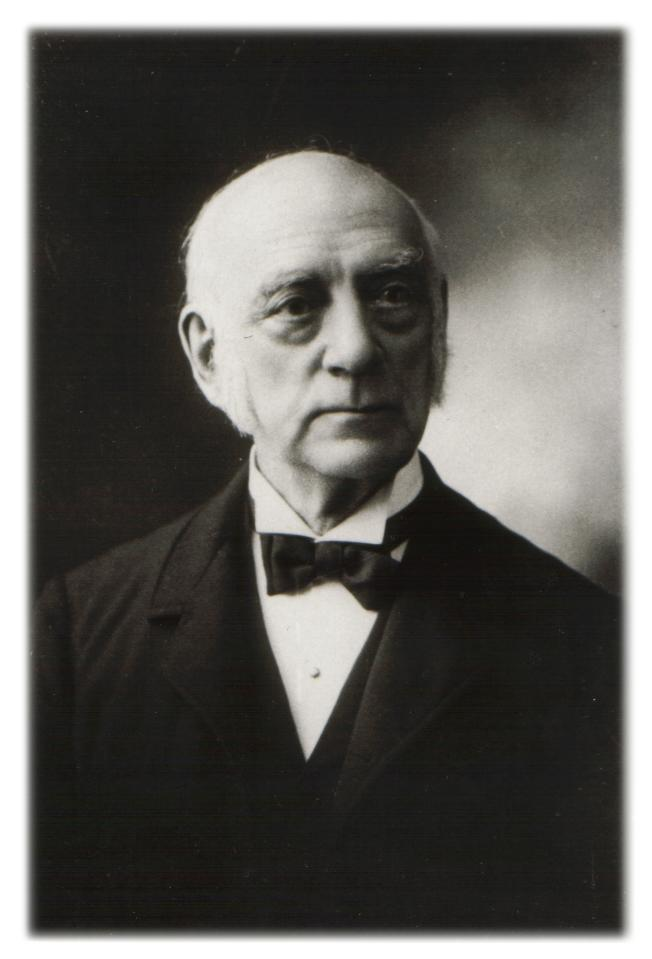
\includegraphics[scale=0.5,trim= 00 00 00 00]{../share/ei/James_Curtis_Hepburn.jpg}}
\\
\end{tabular}


    % label sec:Hepburn
\section{Kunrei System}\jsec{訓令式ローマ字} 
% [o] LABEL
\label{sec:Kunrei}
\label{sec:KunreiSystem}
\label{sec:JapanSystemLatinLetters}
% [o] INDEX
\ifor{Kunrei system}{訓令式ローマ字}{くんれいろうまじ}{Kunrei System}
\ifor{Japan system Latin letters}{日本式ローマ字}{にほんしきろうまじ}{Lateinische Buchstaben des Japanischen Systems}
\ifor{Katakana}{片仮名}{かたかな}{Katakana}
\ifor{Gojūonzu}{五十音図}{ごじゅうおんず}{50 Laute Tafel}
\begin{tabular}{lr}
\begin{minipage}{9.6cm}

The modern \textbf{Kunrei} System {訓令式ローマ字} {【くんれいろうまじ】}  is
the official writing system of Japan. It was confirmed in 1994 by the Cabinet
and is available as ISO 3602:1989. The \textbf{Kunrei} System predecessor was
introduced 1985 by Dr. Aikitsu Tanakadatei ({田中舘愛橘}) as {日本式ローマ字}
{【にほんしきろうまじ】} (Nihon-/Nipponshikiromaji) and tries a more
systematical approach to map \hyperref[sec:Hiragana]{Hiragana} and
\hyperref[sec:Katakana]{Katakana} to equal Roman letters. The {五十音図}
{【ごじゅうおんず】} in the {訓令式ローマ字} is as follows:

\Link \href{http://en.wikipedia.org/wiki/Tanakadate_Aikitsu}{Tanakadate}

\end{minipage}
&
\raisebox{-.5\height}{
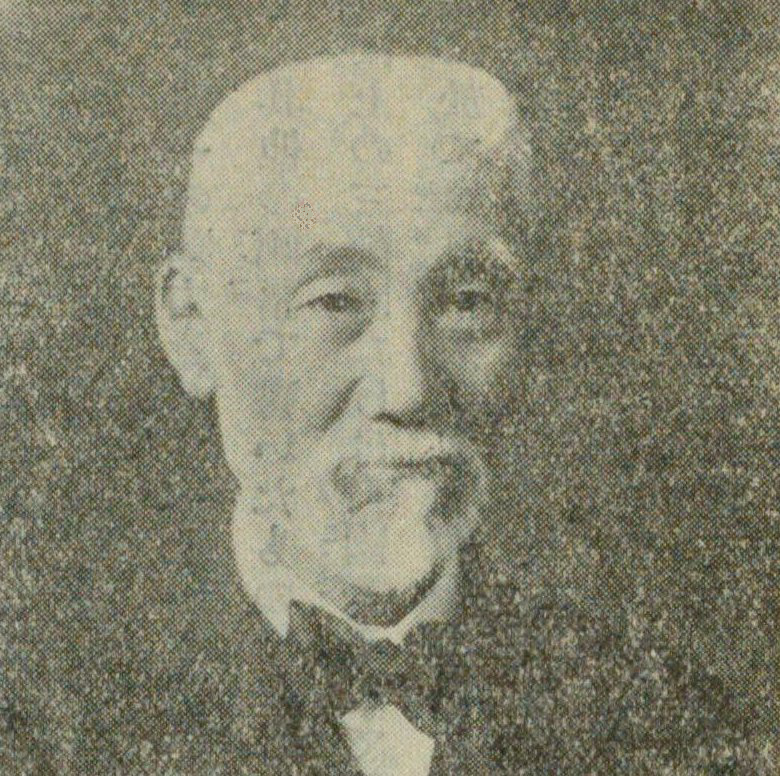
\includegraphics[scale=0.25,trim= 00 00 00 00]{../share/ei/Aikitsu_Tanakadate_r.jpg}}
\\
\end{tabular}


\Info{訓令式ローマ字 - Kunrei System}{
\begin{center}
\begin{tabular}{|c|c|c|c|c|}\hline
   a & i& u& e& o\\\hline
   ka&ki&ku&ke&ko\\\hline
   sa&si&su&se&so\\\hline
   ta&ti&tu&te&to\\\hline
   na&ni&nu&ne&no\\\hline
   ha&hi&hu&he&ho\\\hline
   ma&mi&mu&me&mo\\\hline
   ya&  &yu&  &yo\\\hline
   ra&ri&ru&re&ro\\\hline
   wa&  &  &  & o\\\hline
     &  &  &  & n\\\hline
\end{tabular}
\end{center}
}{true}

Even tough the system is official, many entities (like the train system) are
not using it. They use the Hepburn System.

The {訓令式ローマ字} is not part of this book. Please see \nameref{sec:Hepburn}
(on page \pageref{sec:Hepburn}) for the system in use.
     % label sec:Kunrei
% ---------------------------------------------------------------------------
\section{Diphthong}\jsec{二重母音} \label{sec:Diphthong}
\ithree{diphthong}{二重母音}{Diphthong}
\ithree{diphthong}{にじゅうぼいん}{Diphthong}
\ithree{syllable}{音節}{Silbe}
\ija{「アエ」}
\ija{「アイ」}
\ija{「アウ」}
\ija{「アオ」}
\ija{「ウエ」}
\ija{「ウイ」}
\ija{「オエ」}
\ija{「オイ」}
\ija{「オウ」}

A \textbf{diphthong} {二重母音} {【にじゅうぼいん】} is a sound that is
constructed from two different sounds that glide into each other while
pronouncing and form a \hyperref[sec:Syllable]{syllable}. A \textbf{diphthong}
is made out of vocals.  Examples for a \textbf{diphthong} in Japanese are {姪}
|me.i| and {甥} |o.i|.  Also  {「アエ」}, {「アイ」}, {「アウ」},
{「アオ」}、{「ウエ」}, {「ウイ」}, {「オエ」}, {「オイ」} or {「オウ」} are
likely to appear as a \textbf{diphthong} in normal conversation in Japanese.
However, they becomes vowel connections when it is pronounced slowly and it is
treated as two vowels in the consciousness of the Japanese speaker.
  % label sec:Diphthong
% ---------------------------------------------------------------------------
\section{Mora - モーラ} \label{sec:Mora}

The concept of "mora"  (plural morae or moras; often symbolized μ) is used in
the science of linguistics. It describes a joint unit in pronunciation
(phonology) that constructs a syllable. The definition of a mora can vary.  In
Japanese the detection of morae is comparably simple. The world
{「チョコレート」} for example consist out of the following 5 morae
{「チョ」},{「コ」},{「レ」},{「ー」} and {「ト」} while it consist only out of
four \hyperref[sec:Syllable]{syllables} {(\hyperref[sec:Syllable]{音節}
【おんせつ】)}.

       % label sec:Mora
% ---------------------------------------------------------------------------
\section{Syllable - 音節} \label{sec:Syllable}

A \textbf{syllable} {音節}  {【おんせつ】}  is a phonetic building block for
words. It influences the rhythm of a spoken language. In Western languages a
\textbf{syllable} is made out of one or more letters. In Japanese it is often
one character (of \hyperref[sec:Kana]{Kana}), but not always. For a better
understanding of the Japanese it is important to understand the concept of
\hyperref[sec:Mora]{mora}.

\Link \href{http://en.wikipedia.org/wiki/Syllable}{Syllable}
\Link \href{http://ja.wikipedia.org/wiki/%E9%9F%B3%E7%AF%80}{音節}

   % label sec:Syllable
% ---------------------------------------------------------------------------
\section{Dakuten}\jsec{濁点} \label{sec:Dakuten}
\ithree{diacritic sign}{濁点}{Diakritisches Zeichen}
\ithree{diacritic sign}{だくてん}{Nigorierungszeichen}
\ithree{Umlaut}{ウムラウト}{Umlaut}
\ithree{syllable}{音節}{Silbe}

The \textbf{Dakuten} - Japanese {濁点} {【だくてん】} - is a diacritic sign.
Similar to the German Umlaut.  The {濁点} is referenced colloquial as {点々}
{【てんてん】}.  It us used to in {仮名} \hyperref[sec:Syllable]{syllabaries}
to mark a consonant to be pronounced voiced. Two strokes {「゙」} are used near
the Katakana letter.  For other {濁点}, please see \nameref{sec:Iteration} on
page \pageref{sec:Iteration}.

    % label sec:Dakuten
% ---------------------------------------------------------------------------
\section{Handakuten - 半濁点} \label{sec:Handakuten}

In Japanese two different {濁点} {【だくてん】} are used. The {濁点}  and  the
{半濁点} {【はんだくてん】} has the marker of a little circle {「゚」} and is
therefore colloquially described as {丸} {【まる】} and indicates when the
pronunciation shifts from |h| to |p|.

 % label sec:Handakuten
% ---------------------------------------------------------------------------
\section{Katakana Iteration Marks} \label{sec:Iteration}

As with {漢字} {【かんじ】} also {片仮名} has a iteration mark.  「ヽ」 and its
{濁点} {【だくてん】} form {「ヾ」}. This can only be
found in rare cases. For example the personal name Misuzu 【みすゞ】might
contain this character. And since the difference between the second last
and the last mora is only a change in pronunciation the {濁点} is added.

In vertical writing exist another iteration marker {くの字点} {【くのじてん】}
which consist out of two characters {「〳」+「〵」} and the {濁点} form
is {「〴」+「〵」}

  % label sec:Iteration
% ---------------------------------------------------------------------------
\section{Radical}\jsec{部首}
% [o] LABEL
\label{sec:Radical}
% [o]  INDEX
\ifor{radical}{部首}{ぶしゅ}{Radikal}
\ifor{Kanji}{漢字}{かんじ}{Kanji}

A \textbf{radical} {部首} {【ぶしゅ】} is a root particle or character of a
Sino-Japanese character {漢字} {【かんじ】}. It is the most significant part of
a Sino-Japanese character. The concept was developed in China for Chinese
characters and is today known under the same name {部首} (pinyin: bùshǒu).

There is no general definition what a \textbf{radical} is or how many are
existing and it can vary a lot. The author of a dictionary has the power to
defined what a \textbf{radical} is and how much there will be in that
dictionary.

In more traditional Chinese or Japanese dictionaries a number of 214 or 244
\textbf{radicals} is quite common. However some modern approaches like the
\Link \href{http://www.hadamitzky.de/english/works_books.htm#KD}{\textit{The
Kanji Dictionary} of Marc Spahn and Wolfgang Hadamitzky from 1996} a totally
different number of 79 can be found.

\Note{Note}{\footnotesize Before buying a \hyperref[sec:Kanji]{Kanji}
dictionary, make sure that the \textbf{radical} system used suits your taste.
Sometimes it can be observed that Japanese dictionaries are stricter in the
definition of a \textbf{radical} because a given \hyperref[sec:Kanji]{Kanji}
can only be retrieved via exactly \textit{one} \textbf{radical}. While in many
Chinese dictionaries \textit{every} \textbf{radical} of a Chinese character can
be used to find it. The Japanese approach is of course good in terms of
systematic and didactic for learners, however it can take significant longer to
look up a character by \textbf{radical}.  }

    % label sec:Radical



% ===========================================================================
% END
% ===========================================================================
\end{document}
